\chapter{Hierarchical Phrase-Based Grammar Extraction from Alignment Posterior Probabilities}
\chaptermark{Hiero Extraction from Posteriors}
\label{chap:extractionFromPosteriors}

% TODOFINAL check too much blank space
% TODOFINAL notation for phrase pairs brackets (grep for '(f' for example)
% TODOFINAL grep for {\ (to detect for example {\it )
% TODOFINAL grep for output used as a verb and correct
% TODOFINAL grep \forall and replace comma maybe or find a better way
% TODOFINAL grep for consistent and use it consistently
% TODOFINAL ensure that equations don't go over margin
% TODOFINAL review count assigned to phrase pair in liu et al 2009
% TODOFINAL take look at Jamie's thesis background on HMM word alignment models
% TODOFINAL in grammar pattern section, say which grammars are used for exps
% TODOFINAL read through comments and address left out ones
% TODOFINAL either in this chap or background, add an equation describing the translation model: simply relative frequency src-trg / src
% TODOFINAL check resp. respectively usage
% TODOFINAL throughout refer to background chapter rather than re-citing papers
% TODOFINAL consistent use of hyphens in phrase pairs
% TODOFINAL review grammatical usage of citet citep
% TODOFINAL grep for abbreviations, grep for period and put right spacing
% TODOFINAL uniform notation for phrase pairs: brackets or parenthesis, let's say bracket is better
% TODOFINAL remove all latex compilation warnings
% TODOFINAL (already done ??) somewhere in the introduction, use the convention source and target.
% TODOFINAL try to get rid of htbp in floats and see the outcome
% TODOFINAL get rid of all vertical bars and replace by \mid
% TODOFINAL remove all mbox and replace by text
% TODOFINAL remove all HMM and replace with text{HMM} in equations
% TODOFINAL remove all \bf bu \bm
% TODOFINAL search replace A(i_1, i_2, j_1, j_2) by A(j_1, j_2, i_1, i_2)
% TODOFINAL (already done ??) search replace f_R f_C

In \autoref{chap:hfile}, we have described how to exploit the MapReduce
framework and the HFile format in order to generate very large
translation grammars
and retrieve rules from these grammars efficiently. The main contribution
was at the infrastructure level rather at the modelling level. In this chapter,
we will attempt to improve models for translation grammar extraction.

Standard practice in SMT systems is to decouple the word alignment phase from
the rule extraction phase. Typically, word alignment models are only used to
obtain a set of alignment links, then those alignment links determine
constraints that are followed in the rule extraction
step (see \autoref{sec:hierruleextract}). In
this chapter, we attempt to leverage the information
contained in alignment models by extracting rules from alignment posterior
probabilities~\citep{degispert-pino-byrne:2010:EMNLP}. These statistics are
computed from the HMM alignment model~\citep{vogel-ney-tillmann} and they
are used
both to generate constraints for rule extraction and for translation model
estimation.
%We extract a grammar and estimate a translation model that leads to translation improvements.

This chapter presents two rule extraction methods. With the first method, rules
are extracted from alignment link posterior probabilities. With the second
method, rules are extracted from alignment posterior probabilities
over phrase pairs. We
demonstrate improvements on a medium scale Chinese-English task with these
methods. We also investigate how best to exploit source-to-target and
target-to-source alignment models.

%\section{Notation}
%\label{sec:definitionAndNotation}

%In \autoref{sec:StatisticalMachineTranslationWordAlignment}, we
%have introduced the variable $\bm{a}$, which denotes either
%a set of alignment links or the random variable that defines the word
%alignment model. In this chapter, for clarity, we distinguish these
%two cases. Given a sentence pair $(\bm{f} = f_1^J, \bm{e} = e_1^I)$,
%an alignment \emph{link} is simply a pair $(j, i) \in [1, J] \times [1, I]$.
%We denote $\bm{L}$ to be a set of links for the sentence pair $(\bm{f}, \bm{e})$.
%$\bm{L}$ can be obtained by the Viterbi
%algorithm~\citep{brown-dellapietra-dellapietra-mercer-1993} or maximum a posteriori
%decoding~\citep{matusov-zens-ney:2004:COLING,kumar-och-macherey:2007:EMNLP} and by
%symmetrisation techniques (see \autoref{sec:symmetrisationHeuristics}).
%We also remind definitions from \autoref{sec:hieroTypesOfRules}:
%a \emph{phrase-based} rule is a translation
%rule that contains only terminals in its right hand side;
%a \emph{hierarchical} rule is a translation
%rule that contains at least one nonterminal in its right hand side.

\section{Introduction}
\label{sec:extractionFromPosteriorsIntro}

In state-of-the-art SMT systems, rules are extracted from % TODOFINAL (check abbr)
word-aligned parallel text. The alignments are typically generated by
applying symmetrisation
heuristics (see \autoref{sec:symmetrisationHeuristics}) to Viterbi
alignments (see \autoref{eq:viterbiAlignment}) obtained
from source-to-target and target-to-source word alignment models.
Additional information that these models could provide, such as posterior
probabilities over alignment links, is not used. For example, let us consider
the word-aligned German-English sentence pair in
\autoref{fig:wordalignedSentencePairMistake}.
%
\begin{figure}
  \begin{center}
  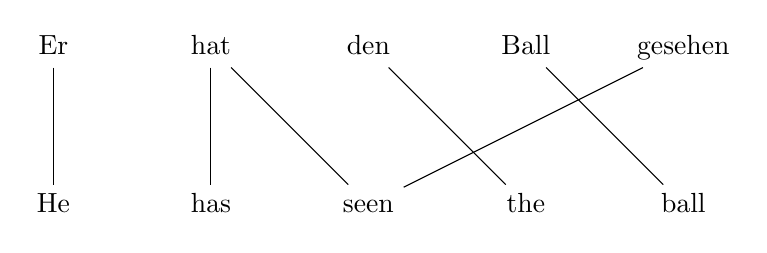
\begin{tikzpicture} [node distance = 2cm, text height=1.5ex, text depth=.25ex]
    % place nodes
    \node (Er) {Er};
    \node [right of = Er] (hat) {hat};
    \node [right of = hat] (den) {den};
    \node [right of = den] (Ball) {Ball};
    \node [right of = Ball] (gesehen) {gesehen};
    %\node [right of = gesehen] (germanDot) {.};
    \node [below of = Er] (He) {He};
    \node [right of = He] (has) {has};
    \node [right of = has] (seen) {seen};
    \node [right of = seen] (the) {the};
    \node [right of = the] (ball) {ball};
    %\node [right of = ball] (englishDot) {.};
    % draw edges
    \draw (Er) -- (He);
    \draw (hat) -- (has);
    \draw (den) -- (the);
    \draw (Ball) -- (ball);
    \draw (gesehen) -- (seen);
    %\draw (germanDot) -- (englishDot);
    % spurious alignment link
    \draw (hat) -- (seen);
  \end{tikzpicture}
  \end{center}
  \caption{German-English word-aligned sentence pair. The spurious alignment
  link between the German word \emph{hat} (\emph{has}) and the English word \emph{seen}
  prevents the phrase pair $\langle$\emph{hat}, \emph{has}$\rangle$ to be extracted from this
  sentence pair.}
  \label{fig:wordalignedSentencePairMistake}
\end{figure}
%
Intuitively, we can tell that
there is a spurious alignment link between the German
word \emph{hat} (\emph{has}) and the
English word \emph{seen}. This link will prevent the extraction of the useful
phrase pair $\langle$\emph{hat}, \emph{has}$\rangle$
from this sentence pair. However, it is
possible that the \emph{posterior probability} of this spurious link according
to the alignment model is relatively low. We hypothesise that posterior
probability information from alignment models is more reliable than the links
obtained from Viterbi alignment.

In this chapter, we use HMM alignment
models (see \autoref{sec:statisticalMachineTranslationHmmAlignmentModel}) to
generate the statistics needed to both extract rules and estimate the
translation models. We hypothesise that this tighter coupling between alignment
and translation models will provide better translation quality.

We will evaluate the grammar we obtain in two ways. First, we will assess the
grammar's ability to generate a reference translation from a source sentence.
This is determined by the type of reordering allowed by the grammar and by
the choice of translations for each source side of a rule. We will then evaluate
translation quality provided by this grammar.

Conceptually, our extraction method consists in extracting all possible phrase
pairs and hierarchical phrase pairs given a sentence pair and selecting only
those that satisfy certain statistical criteria related to alignment posterior
probabilities. For example, we can select phrase pairs that contain a link with
a high posterior probability; or we can select phrase pairs that contain a link
with a high posterior probability and that have a high phrase pair posterior
probability. The selection process determines which rules the grammar will
contain and will therefore define the ability of the grammar to generate a
reference translation given a source sentence. We can also use statistics from
alignment models to estimate translation models in a novel way. In this work, we
will use phrase pair posterior probability instead of integer counts to estimate
translation models.

\section{Related Work}
\label{sec:extractionFromPosteriorRelated}

The limitations of extracting translation rules from Viterbi alignments, i.e.
that potentially useful information from the alignment models is ignored, has
been addressed previously. \citet{venugopal-zollmann-smith-vogel:2008:AMTA}
extract rules from
$n$-best lists of alignments and $n$-best lists of syntactic parses for a
syntax-augmented hierarchical system~\citep{zollmann-venugopal:2006:WMT}.
In the alignment step, an $n$-best list of alignments $\bm{a_1}, ..., \bm{a_n}$ is
produced with posterior probabilities
$p(\bm{a_1} \mid \bm{f}, \bm{e}), ..., p(\bm{a_n} \mid \bm{f}, \bm{e})$. These
posteriors are normalised to produce probabilities
$\hat{p}(\bm{a_1}), ..., \hat{p}(\bm{a_n})$. Similarly, probabilities
$\hat{p}(\bm{\pi_1}), ..., \hat{p}(\bm{\pi_{n'}})$ are obtained
for an $n'$-best list of parses $\bm{\pi_1}, ..., \bm{\pi_{n'}}$. For each alignment
$\bm{a_i}$ and parse $\bm{\pi_j}$, syntax-augmented hierarchical rules are extracted
with a count $\hat{p}(\bm{a_i}) \, \hat{p}(\bm{\pi_j})$.

Alignment $n$-best lists have also been used to create a
structure called
\emph{weighted alignment matrix}~\citep{liu-xia-xiao-liu:2009:EMNLP}.
Probabilities $\hat{p}(\bm{a_1}), ..., \hat{p}(\bm{a_n})$
for $n$-best alignments $\bm{a_1}, ..., \bm{a_n}$ are computed
as previously~\citep{venugopal-zollmann-smith-vogel:2008:AMTA}.
Then, for each word pair $(f_j, e_i)$, the alignment link posterior
probability $p_m(j, i)$ is computed in \autoref{eq:matrixLinkPosterior}.
%
\begin{equation}
  p_m(j, i) = \sum_{k = 1}^n \hat{p}(\bm{a_k}) \delta(\bm{a_k}, i, j)
  \label{eq:matrixLinkPosterior}
\end{equation}
%
$\delta(\bm{a_k}, i, j)$ indicates whether there is a link between $i$ and
$j$ in the alignment $\bm{a_k}$. Given a sentence pair, all phrase
pairs with a maximum source length and a maximum target length that
contain a link with a posterior greater than zero are extracted. The
fractional counts assigned to these phrase pairs are computed in terms
of the link posteriors and then used to estimate the translation models
by relative frequency. The fractional count computation approximates
the posterior probability of all alignments consistent with the phrase
pair. Our method also uses link posterior probabilities
to constrain the extraction but the posteriors are computed
exactly rather than approximated. In addition, posterior probabilities
of consistent alignments is also computed exactly. Finally, our method
is also applied to hierarchical phrase-based translation.

Alignment posterior probabilities without approximation have also been
used.
For a given test set, \citet{deng-and-byrne:2008:ASLP} first extract
phrase pairs in a standard manner. Then, source phrases in the test set
that do not have any corresponding target in the list of extracted
phrase pairs are selected. For each of these source phrases, sentence
pairs where the source phrase occurs are considered. For each such
sentence pair, all target phrases in the target sentence are assigned
phrase pair posterior
probabilities (see \autoref{sec:extractionFromPosteriorsPhrasePair})
according to the
source-to-target and target-to-source alignment models, then ranked
by the geometric average of the two probabilities. The top phrase pair
is retained if its scores are above specific thresholds.
Our definition of phrase pair posterior probabilities and the procedure to compute
them are directly inspired by the work we just described. However, we do not use
the word-to-phrase HMM model but the simpler word-to-word HMM model.
In addition, our method is applied to hierarchical phrase-based grammars
rather than simpler phrase-based grammars. Finally, our grammar
extraction scheme does not consist in
first extracting a standard grammar and then augmenting the grammar with additional rules: we
modify the extraction procedure to directly extract a hierarchical
grammar from alignment link posterior probabilities
or phrase pair posterior probabilities.

\citet{kumar-och-macherey:2007:EMNLP} also use exact computation
of alignment link posteriors in a different application setting.
First, instead of using the Viterbi criterion for word alignment
reminded in \autoref{eq:viterbiCriterion},
%
\begin{equation}
  \bm{\hat{a}} = \argmax_{\bm{a}} p(\bm{f}, \bm{a} \mid \bm{e})
  \label{eq:viterbiCriterion}
\end{equation}
%
the maximum a posteriori criterion~\citep{matusov-zens-ney:2004:COLING}, shown in \autoref{eq:mapCriterion}, is used:
%
\begin{equation}
  \hat{a}_j = \argmax_{i} p(a_j = i \mid \bm{f}, \bm{e})
  \label{eq:mapCriterion}
\end{equation}
%
Then, given a parallel corpus for three languages $F$, $G$, $E$, the
link posteriors for the language pair ($F$, $E$) are computed
in terms of the posteriors for the language pair ($F$, $G$) and ($G$, $E$).
G is called a \emph{bridge} language. The motivation is that
alignments for the $F$-$G$ language pair and the $G$-$E$ language
pair may inform alignment for $F$-$E$. Multiple bridge languages are used
and produce corresponding posterior matrices. The matrices are interpolated
and alignments are extracted for each bridge language and for the
interpolation. Translation gains are obtained in system combination.

We also note approaches to tighter coupling between hierarchical phrase-based
grammars and alignments or even direct modelling of phrase alignment.
\citet{marcu-wong:2002:EMNLP} introduce a joint phrase-based model that
does not make use of word alignments. In this generative model, a sentence
pair is produced by concatenating phrase pairs, or so-called \emph{concepts}.
The authors consider a simpler model with only joint phrase pair translation
probabilities and a more complex model with translation and distortion
probabilities. The parameter are trained with an approximate version of the
expectation-maximisation algorithm~\citep{dempster-laird-rubin:1977:JRSS}.
Experiments demonstrate translation improvements over IBM Model 4.
\citet{birch-callisonburch-osborne-koehn:2006:WMT} constrain this model
in order to be able to apply it to larger parallel corpora. When searching for
a set of phrase pairs to cover a training sentence pair, phrase pairs that
are consistent with the intersection of Viterbi
alignments (see \autoref{sec:symmetrisationHeuristics}) are considered first; other
phrase pairs are considered only when the sentence pair cannot be covered entirely.
Results close to standard phrase-based models are obtained.


\citet{denero-klein:2008:ACL} prove that phrase alignment is an
NP-hard problem. Given a sentence pair $(\bm{f}, \bm{e})$, a bijective phrase
alignment $\bm{a}$ is defined as a bijective mapping between source phrases that
form a partition of $\bm{f}$ and target phrases that form a partition of
$\bm{e}$. A scoring function $\phi$ is also defined that assigns a real-valued
score to any phrase pair $\langle$source phrase, target phrase$\rangle$. The score of a
bijective phrase alignment is simply the product of the scores of its phrase pairs.
Given $(\bm{f}, \bm{e}, \phi)$, the phrase alignment optimisation problem is to find
the best scoring alignment. \citet{denero-klein:2008:ACL} show that this problem
is NP-hard by showing that the corresponding decision problem is NP-complete via
reduction of the SAT problem. We give here an indication of the size of the search
space. The number of possible source partitions is $2^{|\bm{f}| - 1}$.
Given a source partition with $K + 1$ phrases, there are $(K + 1)!$ possible
permutation of the source phrases and $2^{{|e| - 1} \choose K}$ possible target
partitions with $K+1$ phrases. In conclusion, there is little hope to solve
the phrase alignment problem exactly.

\citet{saers-wu:2009:SSST} report an
improvement on a phrase-based system where word alignment has been trained with
an inversion transduction grammar rather than IBM or HMM models.
Phrase alignment is directly modelled with an inversion transduction
grammar. The phrase alignment search space is more restrictive than
the space considered in \citet{denero-klein:2008:ACL} and the
expectation maximisation algorithm can be carried out in $O(n^6)$
where $n$ is the number of tokens in a sentence.
\citet{pauls-klein-chiang-knight:2010:NAACL} also use an
inversion transduction grammar to directly align phrases to nodes in a
string-to-tree model. Bayesian methods have also been developed to induce a
grammar directly from an unaligned parallel
corpus~\citep{blunsom-cohn-osborne:2008:NIPS,blunsom-cohn-dyer-osborne:2009:ACL}.
Finally, \citet{Cmejrek2009} extract rules directly from
bilingual chart parses of the parallel corpus without using word alignments.
We take a different approach in that we aim to start with very strong alignment
models and use them to guide grammar extraction.

Finally, some work on smoothing, which could be complementary to the approach taken
in this thesis, has been conducted to address the
shortcomings of relative frequency estimation for translation models.
\citet{foster-kuhn-johnson:2006:EMNLP} conduct an extensive series of
experiments that either replace the relative frequency estimated phrase table by
a smoothed phrase table or add the smoothed phrase table as a feature and
observe improvement in translation quality.

\section{Rule Extraction}
\label{sec:extractionFromPosteriorsExtraction}

In \autoref{sec:extractionFromPosteriorRelated}, we have reviewed approaches
that ``widen'' the translation pipeline by using alignment $n$-best lists.
We have also reviewed applications of exact computation of alignment posterior
probabilities and attempts to directly model phrase alignment. We will now
describe our grammar extraction methods, based on exact computation of
alignment posterior probabilities under an alignment model.
As in previous work~\citep{hopkins-langmead-vo:2011:WMT},
we first present a general approach that encompasses both standard methods
based on rule extraction from Viterbi alignments as well as our methods.
For clarity of presentation, we first describe our methods in the simpler case
of phrase-based rule extraction, then extend them to hierarchical phrase-based
rule extraction.

\subsection{General Framework for Rule Extraction}
\label{sec:extractionFromPosteriorsExtractionGeneralApproach}

We first describe a general method for the extraction of phrase-based rules.
An extension of this procedure for
hierarchical rules is described in
\autoref{sec:extractionFromPosteriorsExtractionDisjoint}. The algorithm is
described in \autoref{alg:generalRuleXtract}.
%
\begin{figure}
  \begin{algorithmic}[1]
    \Function{ExtractRules}{$f_1^J, e_1^I, \bm{a}$}
      \For{$1 \leq j_1 \leq j_2 \leq J$} \hypertarget{alg:line:sourcePhrase}{} \label{alg:line:sourcePhrase}
        \For{$1 \leq i_1 \leq i_2 \leq I$} \hypertarget{alg:line:targetPhrase}{} \label{alg:line:targetPhrase}
          \If{\Call{SourceConstraints}{$f_{j_1}^{j_2}$} \par
              \hskip\algorithmicindent \hskip\algorithmicindent $\land$ \Call{AlignConstraints}{$f_{j_1}^{j_2}, e_{i_1}^{i_2}, \bm{a}$} \par
              \hskip\algorithmicindent \hskip\algorithmicindent $\land$ \Call{TargetConstraints}{$e_{i_1}^{i_2}$}}
          \hypertarget{alg:line:constraints}{} \label{alg:line:constraints}
            \State{\Call{Extract}{\RT[$X$][$f_{j_1}^{j_2}$][$e_{i_1}^{i_2}$], \Call{Count}{$f_{j_1}^{j_2}, e_{i_1}^{i_2}$}}} \hypertarget{alg:line:extract}{} \label{alg:line:extract}
          \EndIf
        \EndFor
      \EndFor
    \EndFunction
  \end{algorithmic}
  \caption{General procedure for phrase-based rule extraction: both traditional
    rule extraction from Viterbi alignment and our method are instances of this
    procedure.}
  \label{alg:generalRuleXtract}
\end{figure}
%
Given a
sentence pair $(f_1^J, e_1^I)$, for each source index pair $(j_1, j_2)$
defining a source phrase $f_{j_1}^{j_2}$
(\hyperlink{alg:line:sourcePhrase}{line \ref{alg:line:sourcePhrase}}), for each
target index pair $(i_1, i_2)$ defining a target phrase $e_{i_1}^{i_2}$
(\hyperlink{alg:line:targetPhrase}{line \ref{alg:line:targetPhrase}}), if source
constraints, target constraints and
alignment constraints are satisfied
(\hyperlink{alg:line:constraints}{line \ref{alg:line:constraints}}), then the
phrase pair ($f_{j_1}^{j_2}$, $e_{i_1}^{i_2}$) is extracted with a certain
count (\hyperlink{alg:line:extract}{line \ref{alg:line:extract}}): the phrase
pair is added to the list of phrase pairs used in translation, and the count
will be used subsequently to compute translation models by relative frequency.
The purpose
of the constraints is to obtain a manageable number of rules. If we did not
impose constraints, we would extract $\frac{I (I + 1) J (J + 1)}{4}$ (not necessarily distinct) rules
for the sentence pair $(f_1^J, e_1^I)$. During
translation, the decoder would need to apply more pruning, which would
potentially lead to more search errors and a decrease in translation
quality.

We will now refine this general procedure to make it more practical and
closer to a possible implementation.
Let us call the source constraints $\mathcal{C}_S$, the alignment constraints
$\mathcal{C}_A$ and the target constraints $\mathcal{C}_T$. These are
Boolean functions used to select phrase pairs. In practice, source
constraints are checked on the source phrases before looking
at the target phrases. If source constraints are not met, then we need not
consider target phrases for that source phrase.
In addition, target phrases are only considered if they
satisfy alignment constraints with the source phrase and, if they do, we rank
them according to a certain ranking function $\mathcal{R}$. Target constraints also
depend on the ranking $\mathcal{R}$, for example we can decide to keep only a certain
number of target phrases per source phrase. When a phrase pair is extracted, it
is assigned a count which will be used to estimate the source-to-target and
target-to-source translation models. The counting function is called $\mathcal{C}$.
With this notation, we obtain the revised extraction procedure in
\autoref{alg:generalRuleXtractSpecialized}.
%
\begin{figure}
  \begin{algorithmic}[1]
    \Function{ExtractRules}{$f_1^J, e_1^I, \bm{a}$}
      \For{$1 \leq j_1 \leq j_2 \leq J$}
        \If{$\lnot \mathcal{C}_S(f_{j_1}^{j_2})$} \Comment{Source constraints}
          \State{\bf{continue}}
        \EndIf
        \State{$T \gets \emptyset$} \Comment{Sorted target phrases}
        \For{$1 \leq i_1 \leq i_2 \leq I$}
          \If{$\mathcal{C}_A(f_{j_1}^{j_2}, e_{i_1}^{i_2}, \bm{a})$} \Comment{Alignment constraints}
            \State{$T \gets T \cup e_{i_1}^{i_2}$}
          \EndIf
        \EndFor
        \State{\Call{Sort}{$T, \mathcal{R}$}} \Comment{Target phrases ranked according to $\mathcal{R}$}
        \For{$e_{i_1}^{i_2} \in T$}
          \If{$\mathcal{C}_T(e_{i_1}^{i_2}, T)$} \Comment{Target constraints}
            \State{\Call{Extract}{\RT[$X$][$f_{j_1}^{j_2}$][$e_{i_1}^{i_2}$], $\mathcal{C}(f_{j_1}^{j_2}, e_{i_1}^{i_2})$}}
          \EndIf
        \EndFor
      \EndFor
    \EndFunction
  \end{algorithmic}
  \caption{General procedure for phrase-based rule extraction. This version
  is more practical and closer to a possible implementation than the algorithm in \autoref{alg:generalRuleXtract}.
  Source phrases are first considered. Only if source constraints $\mathcal{C}_S$ are satisfied, then
  target phrases are considered. Targets that satisfy alignment constraints $\mathcal{C}_A$ with
  their
  source are ranked by $\mathcal{R}$. Finally, phrase pairs where the target
  satisfies target constraints can be extracted with a certain count $\mathcal{C}$.
  Note that the target constraints implicitly depend on the ranking of the
  targets by $\emph{R}$.}
  \label{alg:generalRuleXtractSpecialized}
\end{figure}
%
We will now describe different rule extraction strategies in terms of
the constraints $\mathcal{C}_S$, $\mathcal{C}_A$, $\mathcal{C_T}$,
the ranking function $\mathcal{R}$ and the counting function $\mathcal{C}$.

\subsection{Extraction from Viterbi Alignment Links}
\label{sec:extractionFromPosteriorsViterbi}

In this section, we describe the standard extraction procedure within
the framework introduced in
\autoref{sec:extractionFromPosteriorsExtractionGeneralApproach}.
Common practice takes a fixed set of word alignment links $\bm{L}$
and extracts
rules from this set. Alignment links $\bm{L}$ are obtained from
the alignment model $\bm{a}$ either by the Viterbi algorithm or
by maximum a posteriori
estimation~\citep{matusov-zens-ney:2004:COLING,kumar-och-macherey:2007:EMNLP}
and possibly using symmetrisation heuristics to combine links obtained
from source-to-target and target-to-source alignment
models (see \autoref{sec:symmetrisationHeuristics}). We can restate this
common approach in the framework proposed in
\autoref{sec:extractionFromPosteriorsExtractionGeneralApproach} and in
\autoref{alg:generalRuleXtractSpecialized} where constraints, ranking and
counting functions are defined as follows:
%
\begin{itemize}
  \item source constraints $\mathcal{C}_S(f_{j_1}^{j_2})$:
%
\begin{equation}
  j_2 - j_1 < s_{\text{max}}
\end{equation}
%
where $s_{\text{max}}$ is a integer threshold defined experimentally.
$s_{\text{max}}$ represents the maximum length of a source phrase.
  \item alignment constraints $\mathcal{C}_A(f_{j_1}^{j_2}, e_{i_1}^{i_2}, \bm{a})$:
%
\begin{equation}
  \Big( \forall (j,i) \in \bm{L}, j \in [j_1, j_2] \Leftrightarrow i \in [i_1,i_2] \Big) \land \Big( \bm{L} \cap [j_1, j_2] \times [i_1, i_2] \neq \emptyset \Big)
  \label{eq:consistencyConstraint}
\end{equation}
%
Alignment constraints have already been described in \autoref{sec:phrasextract} as
the conditions required for phrase pair extraction.
The first bracketed constraint requires that there be no alignment link between a
word inside the phrase pair and a word outside of it. The second
bracketed constraint
requires that
there be at least one alignment link in the phrase pair. Sometimes, an
additional constraint specifies that the boundary words in the phrase pair
should be aligned. In this work, this constraint is not present. % TODOFINAL repeat in background ?
A phrase pair that satisfies \autoref{eq:consistencyConstraint} is said
to be \emph{consistent} with the alignment (see \autoref{sec:phrasextract}).
  \item target constraints $\mathcal{C}_T(e_{i_1}^{i_2}, T)$: no constraint is
    imposed in this work. Target constraints based on length may be imposed
    depending on the implementation.
  \item ranking and counting functions:
%
\begin{equation}
  \mathcal{R}(f_{j_1}^{j_2},e_{i_1}^{i_2}) = \mathcal{C}(f_{j_1}^{j_2},e_{i_1}^{i_2}) = 1
\end{equation}
\end{itemize}
%
The above constraints, ranking and counting functions define the standard
approach to grammar extraction.
In the next sections, we depart from this approach and apply novel functions
to rank and count target-side translations according to their quality in the
context of each parallel sentence, as defined by the word alignment models. We
also depart from common practice in that we do not use a set of links as
alignment constraints. We thus have better control over the number of extracted
rules as well as the relative frequency estimates of the source-to-target and
target-to-source translation models.

\subsection[Extraction from Posteriors Probabilities over Alignment Links]{Extraction from Posteriors Probabilities over \\ Alignment Links}
\label{sec:extractionFromPosteriorsLink}

%We now consider the hidden random variable $\bm{a}$ that models the
%alignment process.
For presentation, we only consider source-to-target
alignment models: the random variable $\bm{a}$ that models the alignment
process
takes values in functions from source
word positions to target word positions. However, it it possible to apply
our method with any directional alignment model.
We will use the link
posterior probability $p(a_j = i \mid f_1^J, e_1^I)$ to guide
rule extraction. This statistic expresses how likely it is that
a word $f_j$ in source position $j$ and a word $e_i$ in
target position $i$ are aligned given the sentence pair $(f_1^J,e_1^I)$.
The link posterior probability can be computed efficiently for
Model 1, Model 2 and HMM. In our experiments, we only use the HMM model
to compute link posteriors but comparisons between link posteriors obtained
from various models may be interesting in the future. We will derive
a closed form solution for these models to compute the link posterior
probability.
Applying the definition of conditional
probability, we obtain the general form of the link posterior probability in
\autoref{eq:linkposdef}.
%
\begin{equation} \label{eq:linkposdef}
  p(a_{j_0} = i_0 \mid f_1^J, e_1^I) = \frac{p(a_{j_0}=i_0,f_1^J \mid e_1^I)}{p(f_1^J \mid e_1^I)}
\end{equation}
%
Using \autoref{eq:linkposdef}, we will now derive the link posterior probability
$p_{M_1}(a_{j_0} = i_0 \mid f_1^J, e_1^I)$ for Model 1,
$p_{M_2}(a_{j_0} = i_0 \mid f_1^J, e_1^I)$ for Model 2 and
$p_{\text{HMM}}(a_{j_0} = i_0 \mid f_1^J, e_1^I)$ for the HMM model.

\subsubsection{Link Posterior Probability for Model 1}

Let us derive $p_{M_1}(a_{j_0} = i_0 \mid f_1^J, e_1^I)$,
the link posterior probability under Model 1. We use the notation
from~\citep{brown-dellapietra-dellapietra-mercer-1993}, where $t$ is
the word-to-word translation table and $\varepsilon$ is a constant. We compute the
numerator from
\autoref{eq:linkposdef} by marginalising over all possible alignments and
inverting sum and product signs to obtain \autoref{eq:linkposM1Numerator}:
%
\begin{align}
  & p_{M_1}(a_{j_0}=i_0,f_1^J \mid e_1^I) \nonumber \\
  &= \sum_{a_1 = 0}^{I} ... \sum_{a_{j_0-1} = 0}^{I} \sum_{a_{j_0+1} = 0}^{I} ... \sum_{a_J = 0}^{I} p_{M_1}(a_1 ... a_{j_0-1} i_0 a_{j_0+1} ... a_J,f_1^J \mid e_1^I) \nonumber \\
  &= \sum_{a_1 = 0}^{I} ... \sum_{a_{j_0-1} = 0}^{I} \sum_{a_{j_0+1} = 0}^{I} ... \sum_{a_J = 0}^{I} \frac{\varepsilon}{(1+I)^J} t(f_{j_0} \mid e_{i_0}) \prod_{\substack{j = 1 \\ j \neq j_0}}^J t(f_j \mid e_{a_j}) \nonumber \\
  &= \frac{\varepsilon}{(1+I)^J} t(f_{j_0} \mid e_{i_0}) \prod_{\substack{j = 1 \\ j \neq j_0}}^J \sum_{i=0}^I t(f_j \mid e_i) \label{eq:linkposM1Numerator}
\end{align}
%
We compute the denominator from \autoref{eq:linkposdef}
similarly (see Equation (15)
in~\citep{brown-dellapietra-dellapietra-mercer-1993}) and obtain
\autoref{eq:linkposM1Denominator}:
%
\begin{equation} \label{eq:linkposM1Denominator}
  p_{M_1}(f_1^J \mid e_1^I) = \frac{\varepsilon}{(1+I)^J} \prod_{j=1}^J \sum_{i=0}^I t(f_j \mid e_i)
\end{equation}
%
After simplification, we obtain \autoref{eq:linkposM1} from
\autoref{eq:linkposM1Numerator} and \autoref{eq:linkposM1Denominator}:
%
\begin{equation} \label{eq:linkposM1}
  p_{M_1}(a_{j_0} = i_0 \mid f_1^J, e_1^I) = \frac{t(f_{j_0}|e_{i_0})}{\sum_{i=0}^I t(f_{j_0}|e_i)}
\end{equation}
%

\subsubsection{Link Posterior Probability for Model 2}
We apply the same method to compute $p_{M_2}(a_{j_0} = i_0 \mid f_1^J, e_1^I)$, the
link posterior probability for Model 2. We also use
notation from~\citep{brown-dellapietra-dellapietra-mercer-1993} but
we replace the notation for the alignment probability $a(i \mid j, J, I)$
by $p_a(i \mid j, J, I)$ for clarity.
We compute the numerator from \autoref{eq:linkposdef} in
\autoref{eq:linkposM2Numerator}:
%
\begin{align}
  & p_{M_2}(a_{j_0}=i_0,f_1^J \mid e_1^I) \nonumber \\
  &= \sum_{a_1 = 0}^{I} ... \sum_{a_{j_0-1} = 0}^{I} \sum_{a_{j_0+1} = 0}^{I} ... \sum_{a_J = 0}^{I} p_{M_2}(a_1 ... a_{j_0-1} i_0 a_{j_0+1} ... a_J,f_1^J \mid e_1^I) \nonumber \\
  &= \sum_{a_1 = 0}^{I} ... \sum_{a_{j_0-1} = 0}^{I} \sum_{a_{j_0+1} = 0}^{I} ... \sum_{a_J = 0}^{I} \varepsilon \ p_a(i_0 \mid j_0, J, I) \ t(f_{j_0} \mid e_{i_0}) \nonumber \\
  & \; \; \qquad \qquad \qquad \qquad \qquad \qquad \prod_{\substack{j = 1 \\ j \neq j_0}}^J p_a(a_j \mid j, J, I) \ t(f_j \mid e_{a_j}) \nonumber \\
  &= \varepsilon \ p_a(i_0 \mid j_0, J, I) \ t(f_{j_0} \mid e_{i_0}) \prod_{\substack{j = 1 \\ j \neq j_0}}^J \sum_{i=0}^I p_a(i \mid j, J, I) \ t(f_j \mid e_i) \label{eq:linkposM2Numerator}
\end{align}
%
We compute the denominator from \autoref{eq:linkposdef} similarly and obtain
\autoref{eq:linkposM2Denominator}:
%
\begin{equation} \label{eq:linkposM2Denominator}
  p_{M_2}(f_1^J \mid e_1^I) = \varepsilon \ \prod_{j=1}^J \sum_{i=0}^I p_a(i \mid j, J, I) \ t(f_j \mid e_i)
\end{equation}
%
After simplification, we obtain \autoref{eq:linkposM2} from
\autoref{eq:linkposM2Numerator} and \autoref{eq:linkposM2Denominator}.
%
\begin{equation} \label{eq:linkposM2}
  p_{M_2}(a_{j_0} = i_0 \mid f_1^J, e_1^I) = \frac{p_a(i_0 \mid j_0, J, I) \ t(f_{j_0} \mid e_{i_0})}{\sum_{i=0}^I p_a(i \mid j_0, J, I) \ t(f_{j_0} \mid e_i)}
\end{equation}
%

\subsubsection{Link Posterior Probability for the HMM Model}
\label{sec:linkPosteriorHMM}
We now derive $p_{\text{HMM}}(a_{j_0} = i_0 | f_1^J, e_1^I)$, the link posterior
probability for the HMM
model~\citep{vogel-ney-tillmann,rabiner:1989:IEEE}. These derivations
are standard once we realise that the observed sequence is the source
sentence $f_1^J$, the hidden sequence is $a_1^J$ and that in addition
to standard presentations of HMM, all probabilities are conditioned on
the target sentence $e_1^I$.
We compute the numerator from \autoref{eq:linkposdef} in
\autoref{eq:linkposHMMNumerator}:
%
\begin{align}
  p_{\text{HMM}}(a_{j_0} = i_0, f_1^J \mid e_1^I) &= p_{\text{HMM}}(a_{j_0} = i_0, f_1^{j_0}, f_{j_0 + 1}^J \mid e_1^I) \nonumber \\
                                               &= p_{\text{HMM}}(f_{j_0 + 1}^J \mid a_{j_0} = i_0, f_1^{j_0}, e_1^I) \ p_{\text{HMM}}(a_{j_0} = i_0, f_1^{j_0} \mid e_1^I) \nonumber \\
                                               &= p_{\text{HMM}}(f_{j_0 + 1}^J \mid a_{j_0} = i_0, e_1^I) \ p_{\text{HMM}}(a_{j_0} = i_0, f_1^{j_0} \mid e_1^I) \nonumber \\
                                               &= \beta_{j_0}(i_0) \ \alpha_{j_0}(i_0) \label{eq:linkposHMMNumerator}
\end{align}
%
where $\beta_{j_0}(i_0)$ and $\alpha_{j_0}(i_0)$ are respectively
the backward and forward HMM probabilities defined in \autoref{eq:backwardForward}:
%
\begin{equation}
  \begin{split}
    \beta_{j}(i)  &= p_{\text{HMM}}(f_{j + 1}^J \mid a_{j} = i, e_1^I) \\
    \alpha_{j}(i) &= p_{\text{HMM}}(a_{j} = i, f_1^{j} \mid e_1^I)
  \end{split}
  \label{eq:backwardForward}
\end{equation}
%
The forward and backward probabilities can be computed recursively as
shown in \autoref{eq:forwardRecursion} and \autoref{eq:backwardRecursion}:
%
\begin{align}
  \alpha_{j}(i) &= p_{\text{HMM}}(a_{j} = i, f_1^{j} \mid e_1^I) \nonumber \\
                &= \sum_{k = 0}^I p_{\text{HMM}}(a_{j} = i, a_{j - 1} = k, f_1^{j - 1}, f_j \mid e_1^I) \nonumber \\
                &= \sum_{k = 0}^I p_{\text{HMM}}(f_j \mid a_j = i, a_{j - 1} = k, f_1^{j-1}, e_1^I) \ p_{\text{HMM}}(a_{j} = i, a_{j - 1} = k, f_1^{j - 1} \mid e_1^I) \nonumber \\
                &= \sum_{k = 0}^I p_{\text{HMM}}(f_j \mid e_i) \ p_{\text{HMM}}(a_{j} = i \mid a_{j - 1} = k, f_1^{j - 1}, e_1^I) \ p_{\text{HMM}}(a_{j - 1} = k, f_1^{j - 1} \mid e_1^I) \nonumber \\
                &= \sum_{k = 0}^I p_{\text{HMM}}(f_j \mid e_i) \ p_{\text{HMM}}(a_{j} = i \mid a_{j - 1} = k, I) \ \alpha_{j - 1}(k) \label{eq:forwardRecursion} \\
  \beta_{j}(i)  &= p_{\text{HMM}}(f_{j + 1}^J \mid a_{j} = i, e_1^I) \nonumber \\
                &= \sum_{k = 0}^I p_{\text{HMM}}(f_{j+2}^J, a_{j + 1} = k, f_{j + 1} \mid a_j = i, e_1^I) \nonumber \\
                &= \sum_{k = 0}^I p_{\text{HMM}}(f_{j+2}^J \mid a_{j + 1} = k, f_{j + 1}, a_j = i, e_1^I) \ p_{\text{HMM}}(a_{j + 1} = k, f_{j + 1} \mid a_j = i, e_1^I) \nonumber \\
                &= \sum_{k = 0}^I p_{\text{HMM}}(f_{j+2}^J \mid a_{j + 1} = k, e_1^I) \ p_{\text{HMM}}(f_{j + 1} \mid a_{j + 1} = k, a_j = i, e_1^I) \nonumber \\
                & p_{\text{HMM}}(a_{j + 1} = k \mid a_j = i, e_1^I) \nonumber \\
                &= \sum_{k = 0}^I \beta_{j + 1}(k) \ p_{\text{HMM}}(f_{j + 1} \mid e_k) \ p_{\text{HMM}}(a_{j + 1} = k \mid a_j = i, I) \label{eq:backwardRecursion}
\end{align}
%
The denominator from \autoref{eq:linkposdef} is computed in
\autoref{eq:linkposHMMDenominator}:
%
\begin{align}
  p_{\text{HMM}}(f_1^J \mid e_1^I) &= \sum_{k = 0}^I p_{\text{HMM}}(a_J = k, f_1^J \mid e_1^I) \nonumber \\
                                &= \sum_{k = 0}^I \alpha_J(k) \label{eq:linkposHMMDenominator}
\end{align}
%
%
%We now derive the link posterior probability for the WPHMM Model.
%TODONEVER(should refer here to a background section for notation, etc.)
% TODONEVER: link posteriors for WPHMM and phrase pair posteriors
%

We will use the link posterior probabilities under the HMM model
in order to define constraints, ranking and counting functions.

\subsubsection{Constraints, Ranking and Counting Functions from HMM Link Posterior Probabilities}

We use HMM link posterior probabilities computed in \autoref{sec:linkPosteriorHMM}
in order to define constraints, ranking and counting functions:
%
\begin{itemize}
  \item source constraints $\mathcal{C}_S(f_{j_1}^{j_2})$:
%
\begin{equation}
  j_2 - j_1  < s_{\text{max}}
\end{equation}
%
This is the same constraint as defined for standard Viterbi extraction in
\autoref{sec:extractionFromPosteriorsViterbi}.
  \item alignment constraints $\mathcal{C}_A(f_{j_1}^{j_2}, e_{i_1}^{i_2}, \bm{a})$:
%
\begin{align}
 & \exists (j,i) \in [j_1,j_2] \times [i_1,i_2], p(a_j = i \mid f_1^J,e_1^I) > \lambda \label{eq:firstAlignmentConstraintHmmLinkPosterior} \\
 & \forall (j,i) \in [1, J] \times [1, I] \cap \{(j,i): p(a_j = i \mid f_1^J,e_1^I) > \lambda\} \label{eq:secondAlignmentConstraintHmmLinkPosterior} \\
 & \hspace{3em} j \in [j_1, j_2] \Leftrightarrow i \in [i_1, i_2] \nonumber
\end{align}
%
where $\lambda$ is a threshold defined experimentally. Intuitively,
$\lambda$ is a high link posterior probability.
The first constraint (\autoref{eq:firstAlignmentConstraintHmmLinkPosterior}) means that we require at least one link with a
high posterior probability in the phrase pair considered. The second
constraint (\autoref{eq:secondAlignmentConstraintHmmLinkPosterior}) means that there should be no link with a high posterior probability
that be inconsistent with the phrase pair. Note that these constraints are
identical to the Viterbi alignment constraints defined
in \autoref{sec:extractionFromPosteriorsViterbi} if we choose $\bm{L}$ to be the
set of all links with high posterior defined in \autoref{eq:linksWithHighPosterior}:
%
\begin{equation}
  \bm{L} = \{(j, i) \in [1, J] \times [1, I]: p(a_j = i \mid f_1^J,e_1^I) > \lambda\}
  \label{eq:linksWithHighPosterior}
\end{equation}
%
Also note that the second
constraint does not consider links to the null
word (see \autoref{sec:StatisticalMachineTranslationWordAlignment}) relevant.
This is because we do not need to include the null word
in a translation rule.
  \item target constraints $\mathcal{C}_T(e_{i_1}^{i_2}, T)$: we pick the
    first $k$ translation candidates according to the ranking
    function $\mathcal{R}$.
  \item ranking function:
%
\begin{equation} \label{eq:linkPosRanking}
  \mathcal{R}(f_{j_1}^{j_2},e_{i_1}^{i_2}) = \prod_{j=j_1}^{j_2} \sum_{i=i_1}^{i_2} \frac{p(a_j = i \mid f_1^J,e_1^I)}{i_2-i_1+1}
\end{equation}
%
This ranking function is very similar to the score used for lexical features
described in \autoref{sec:features}. Here,
we use link posteriors instead of Model 1 translation probabilities. This
function favours short target phrases, therefore we do not use it as a counting
function. Preliminary experiments found that this function is not appropriate for
counting rules and that it gives poor results. We therefore use the same counting
function as in standard practice described in
\autoref{sec:extractionFromPosteriorsViterbi}.
  \item counting function:
%
\begin{equation}
  \mathcal{C}(f_{j_1}^{j_2},e_{i_1}^{i_2}) = 1
\end{equation}
%
\end{itemize}

We have described rule extraction from alignment link posterior
probabilities. Next, we will describe rule extraction from alignment
posterior probabilities over phrase pairs. This method will use the
same source constraints, alignment constraints and target constraints
but different ranking and counting functions.

\subsection{Extraction from Posteriors over Phrase Pairs}
\label{sec:extractionFromPosteriorsPhrasePair}

In the previous section, we defined and gave closed form solutions to
alignment link posterior probabilities for Model 1, Model 2 and the HMM model.
We can also define alignment posterior probabilities over phrase pairs. Let us
consider the phrase pair $\langle f_{j_1}^{j_2}, e_{i_1}^{i_2} \rangle$ in the
sentence pair $(f_1^J, e_1^I)$. In
\autoref{eq:alignmentConsistentDefinition}, we define
$A(j_1, j_2; i_1, i_2)$, the set of alignments that have no links between
inside the phrase pair and outside the phrase pair:
%
\begin{equation}
  A(j_1, j_2;i_1, i_2) = \{a_1^J : a_j \in [i_1, i_2] \Leftrightarrow j \in [j_1,j_2] \}
  \label{eq:alignmentConsistentDefinition}
\end{equation}
%
Alignments in $A(j_1, j_2;i_1, i_2)$ satisfy the consistency constraint
defined in \autoref{eq:consistencyConstraint}
but do not require a link in $[j_1, j_2] \times [i_1, i_2]$.
The posterior probability of these alignments given the sentence
pair is defined in \autoref{eq:phrasePairPosteriorDefinition}:
%
\begin{equation}
  \begin{split}
  p(A(j_1, j_2; i_1, i_2) \mid e_1^I, f_1^J) &= \frac{p(f_1^J, A(j_1, j_2; i_1, i_2) \mid e_1^I)}{p(f_1^J \mid e_1^I)} \\
                                          &= \frac{\sum_{a_1^J \in A(j_1, j_2; i_1, i_2)} p(f_1^J,a_1^J \mid e_1^I)}{\sum_{a_1^J} p(f_1^J,a_1^J \mid e_1^I)}
  \end{split}
  \label{eq:phrasePairPosteriorDefinition}
\end{equation}
%
We call this quantity the \emph{phrase pair posterior probability}.
We will now derive formula for the phrase pair posterior probability in the
case of Model 1, Model 2 and the HMM Model. Again, experiments only use phrase pair
posteriors computed from the HMM model, but comparing those with the posteriors
obtained from Model 1 and Model 2 may be interesting for future research.

\subsubsection{Phrase Pair Posterior Probability for Model 1}

Let us first define $J_{\text{in}}$, $J_{\text{out}}$, $I_{\text{in}}$ and
$I_{\text{out}}$ in \autoref{eq:iInsideOutside} for a set of indices
$i_1$, $i_2$, $j_1$, $j_2$:
%
\begin{equation}
\begin{split}
  J_{\text{in}} &= [j_1, j_2] \\
  J_{\text{out}} &= [1,J] \setminus J_{\text{in}} \\
  I_{\text{in}} &= [i_1, i_2] \\
  I_{\text{out}} &= [0, I] \setminus I_{\text{in}}
\end{split}
\label{eq:iInsideOutside}
\end{equation}
%
For Model 1, the numerator from \autoref{eq:phrasePairPosteriorDefinition} is
obtained in \autoref{eq:phrasePairPosteriorModel1Numerator}:
%
\begin{align}
  & \sum_{a_1^J \in A(j_1, j_2; i_1, i_2)} p_{M_1}(f_1^J, a_1^J \mid e_1^I) \nonumber \\
  &= \sum_{a_1 \in I_{\text{out}}} ... \sum_{a_{j_1-1} \in I_{\text{out}}} \sum_{a_{j_1} \in I_{\text{in}}} ... \sum_{a_{j_2} \in I_{\text{in}}} \sum_{a_{j_2 + 1} \in I_{\text{out}}} ... \sum_{a_J \in I_{\text{out}}} p_{M_1}(a_1^J, f_1^J \mid e_1^I) \nonumber \\
  &= \sum_{a_1 \in I_{\text{out}}} ... \sum_{a_{j_1-1} \in I_{\text{out}}} \sum_{a_{j_1} \in I_{\text{in}}} ... \sum_{a_{j_2} \in I_{\text{in}}} \sum_{a_{j_2 + 1} \in I_{\text{out}}} ... \sum_{a_J \in I_{\text{out}}} \frac{\varepsilon}{(1+I)^J} \prod_{j = 1}^J t(f_j \mid e_{a_j}) \nonumber \\
  &= \frac{\varepsilon}{(1+I)^J} \ \left( \prod_{j \in J_{\text{out}}} \sum_{i \in I_{\text{out}}} t(f_j \mid e_i) \right) \ \left( \prod_{j \in J_{\text{in}}} \sum_{i \in I_{\text{in}}} t(f_j \mid e_i) \right)
  \label{eq:phrasePairPosteriorModel1Numerator}
\end{align}
%
The denominator from \autoref{eq:phrasePairPosteriorDefinition} has already been
computed in \autoref{eq:linkposM1Denominator}.
Simplifying \autoref{eq:phrasePairPosteriorModel1Numerator} and
\autoref{eq:linkposM1Denominator}, we obtain
\autoref{eq:phrasePairPosteriorModel1}:
%
\begin{align}
  & p_{M_1}(A(j_1, j_2; i_1, i_2) \mid e_1^I, f_1^J) \nonumber \\
  &= \left( \prod_{j \in J_{\text{out}}} \sum_{i \in I_{\text{out}}} \frac{t(f_j \mid e_i)}{\sum_{i' = 0}^I t(f_{j} \mid e_{i'})} \right)  \left( \prod_{j \in J_{\text{in}}} \sum_{i \in I_{\text{in}}} \frac{t(f_j \mid e_i)}{\sum_{i' = 0}^I t(f_{j} \mid e_{i'})} \right) \nonumber \\
  &= \left( \prod_{j \in J_{\text{out}}} \sum_{i \in I_{\text{out}}} p_{M_1}(a_j = i \mid f_1^J, e_1^I) \right) \left( \prod_{j \in J_{\text{in}}} \sum_{i \in I_{\text{in}}} p_{M_1}(a_j = i \mid f_1^J, e_1^I) \right)
  \label{eq:phrasePairPosteriorModel1}
\end{align}
%

\subsubsection{Phrase Pair Posterior Probability for Model 2}

To avoid repetition, we skip the derivation which is analogous to
the derivation for Model 1. We obtain the phrase pair posterior in
\autoref{eq:phrasePairPosteriorModel2}:
%
\begin{align}
  & p_{M_2}(A(j_1, j_2; i_1, i_2) \mid e_1^I, f_1^J) \nonumber \\
  &= \left( \prod_{j \in J_{\text{out}}} \sum_{i \in I_{\text{out}}} p_{M_2}(a_j = i \mid f_1^J, e_1^I) \right) \left( \prod_{j \in J_{\text{in}}} \sum_{i \in I_{\text{in}}} p_{M_2}(a_j = i \mid f_1^J, e_1^I) \right)
  \label{eq:phrasePairPosteriorModel2}
\end{align}
%

\subsubsection{Phrase Pair Posterior Probability for HMM}

Let us now compute the phrase pair posterior probability for the HMM model. The
denominator from \autoref{eq:phrasePairPosteriorDefinition} can be computed using
the forward algorithm while the numerator can be computed using a modified
forward algorithm~\citep{deng:2005:PHD}. Let us define $\tilde{\alpha}_j(i)$, the
modified forward probability in \autoref{eq:modifiedForwardProbabilityDefinition}:
%
\begin{equation}
  \tilde{\alpha}_j(i) = p_{\text{HMM}}(A(j_1,j_2;i_1,i_2), f_1^j, a_j=i \mid e_1^I)
  \label{eq:modifiedForwardProbabilityDefinition}
\end{equation}
%
The numerator from \autoref{eq:phrasePairPosteriorDefinition} can be computed
in \autoref{eq:phrasePairPosteriorHMMNumerator}:
%
\begin{equation}
  p(A(j_1, j_2; i_1, i_2), f_1^J \mid e_1^I) = \sum_{i=0}^I \tilde{\alpha}_J(i)
  \label{eq:phrasePairPosteriorHMMNumerator}
\end{equation}
%
The denominator from \autoref{eq:phrasePairPosteriorDefinition} can be computed
using the regular forward probability in
\autoref{eq:phrasePairPosteriorHMMDenominator}:
%
\begin{equation}
  p(f_1^J \mid e_1^I) = \sum_{i=0}^I \alpha_J(i)
  \label{eq:phrasePairPosteriorHMMDenominator}
\end{equation}
%
Like the regular forward probability, the modified forward probability can also
be computed recursively. We can also write the modified forward probability as
in \autoref{eq:rewriteModifiedForwardProbability}:
%
\begin{equation}
  \begin{split}
  \tilde{\alpha}_j(i) &= p_{\text{HMM}}(A(j_1,j_2;i_1,i_2), f_1^j, a_j=i \mid e_1^I) \\
                      &= \sum_{a_1^{j} \in A(j_1,j_2;i_1,i_2)} p_{\text{HMM}}(a_1^{j-1}, f_1^j, a_j=i \mid e_1^I) \\
                      &= \sum_{\substack{a_1^{j} \in A(j_1,j_2;i_1,i_2) \\ a_j=i}} p_{\text{HMM}}(a_1^{j-1}, f_1^j, a_j=i \mid e_1^I)
  \end{split}
  \label{eq:rewriteModifiedForwardProbability}
\end{equation}
%
The computation of $\tilde{\alpha}_j(i)$ is by a constrained forward algorithm where
the constraint is given in \autoref{eq:modifiedForwardConstraints}. This is because
an alignment in $A(j_1,j_2;i_1,i_2)$  cannot have a link from inside the phrase
pair to outside the phrase pair (see \autoref{eq:alignmentConsistentDefinition}):
%
\begin{equation}
  \forall (j, i) \in J_{\text{out}} \times I_{\text{in}} \cup J_{\text{in}} \times I_{\text{out}}, \tilde \alpha_j(i) = 0
  \label{eq:modifiedForwardConstraints}
\end{equation}
%
For a link $(j, i) \in J_{\text{out}} \times I_{\text{out}} \cup J_{\text{in}} \times I_{\text{in}}$ that satisfies the constraint from
\autoref{eq:modifiedForwardConstraints}, we can derive the modified
forward probability in \autoref{eq:modifiedForwardRecursion}:
%
\begin{align}
  \tilde{\alpha}_j(i) &= p_{\text{HMM}}(A(j_1, j_2; i_1, i_2), f_1^j, a_j=i \mid e_1^I) \nonumber \\
                      &= \sum_{a_1^{j-1} \in A(j_1, j_2; i_1, i_2)}
                         p_{\text{HMM}}(f_j, f_1^{j-1},  a_j=i, a_1^{j-1} \mid e_1^I) \nonumber \\
                      &= \sum_{a_1^{j-1} \in A(j_1, j_2; i_1, i_2)}
                         p_{\text{HMM}}(f_j \mid f_1^{j-1},  a_j=i, a_1^{j-1}, e_1^I) \times \nonumber \\
                      & \hspace{7.7em} p_{\text{HMM}}(a_j=i \mid f_1^{j-1}, a_1^{j-1}, e_1^I) \times \nonumber \\
                      & \hspace{7.7em} p_{\text{HMM}}(f_1^{j-1}, a_1^{j-1} \mid e_1^I) \nonumber \\
                      &= p_{\text{HMM}}( f_j \mid e_i ) 
                         \sum_{a_1^{j-1} \in A(j_1, j_2; i_1, i_2)}
                         p_{\text{HMM}}(a_j=i \mid a_{j-1}, I) \
                         p_{\text{HMM}}(f_1^{j-1},  a_1^{j-1} \mid e_1^I) \nonumber \\
                      &= p_{\text{HMM}}(f_j \mid e_i) \
                         \sum_{k=0}^I \sum_{\substack{a_1^{j-1} \in A(j_1, j_2; i_1, i_2) \\ a_{j-1} = k}}
                         p_{\text{HMM}}(a_j=i \mid a_{j-1} = k, I) \nonumber \\
                      & \hspace{15.2em} p_{\text{HMM}}(f_1^{j-1},  a_{j-1} = k,  a_1^{j-2} \mid e_1^I) \nonumber \\
                      &= p_{\text{HMM}}(f_j \mid e_i) \
                         \sum_{k = 0}^I
                         p_{\text{HMM}}(a_j = i \mid a_{j-1} = k, I) \nonumber \\
                      & \hspace{4.7em} \sum_{\substack{a_1^{j-1} \in A(j_1, j_2; i_1, i_2) \\ a_{j-1} = k}}
                         p_{\text{HMM}}(f_1^{j-1},  a_{j-1} = k,  a_1^{j-2} \mid e_1^I) \nonumber \\
                      &= p_{\text{HMM}}(f_j \mid e_i) \
                         \sum_{k = 0}^I
                         p_{\text{HMM}}(a_j=i \mid a_{j-1} = k, I) \; \tilde \alpha_{j-1}(k)
                         \label{eq:modifiedForwardRecursion}
\end{align}
%
We will use the phrase pair posterior probabilities under the HMM model
in order to define ranking and counting functions.

\subsubsection{Constraints, Ranking and Counting Functions from HMM Link and Phrase Posterior Probabilities}

In order to keep the size of the rule set manageable, we use
the same source constraints, alignment constraints and target constraints
as for link posterior extraction defined in
\autoref{sec:extractionFromPosteriorsLink}.
We use the phrase pair posterior probabilities under the HMM model both for ranking
and scoring
extracted rules. This approach assigns a fractional count to each extracted
rule, which allows finer estimation of the source-to-target and target-to-source
translation models.  The ranking and counting functions
are defined in \autoref{eq:rankingCountingPhrasePairExtraction}:
%
\begin{equation}
  \mathcal{R}(f_{j_1}^{j_2},e_{i_1}^{i_2}) = \mathcal{C}(f_{j_1}^{j_2},e_{i_1}^{i_2}) = p_{\text{HMM}}(A(j_1, j_2; i_1, i_2) \mid f_1^j, e_1^J)
  \label{eq:rankingCountingPhrasePairExtraction}
\end{equation}

Under the framework described in
\autoref{sec:extractionFromPosteriorsExtractionGeneralApproach}, we have
described standard rule extraction from Viterbi alignments and two novel
approaches to rule extraction based on link posterior probabilities and
phrase pair posterior probabilities. In order to expose concepts with more
clarity, we have restricted the presentation
to the extraction of phrase based rules as opposed to hierarchical rules.
We will now show how to generalise the techniques presented so far to
the extraction of hierarchical rules.

\subsection{Hierarchical Rule Extraction}
\label{sec:extractionFromPosteriorsExtractionDisjoint}

In this section, we extend the techniques presented so far to hierarchical
rule extraction. In order to avoid repetition, we describe these
techniques for the rule pattern
$\langle w X w, w X w \rangle$
only (see \autoref{sec:constraintsOnHierarhicalGrammars} for the
definition of patterns). We first rewrite the algorithm in
\autoref{alg:generalRuleXtractSpecialized} into the algorithm in
\autoref{alg:generalRuleXtractSpecializedHierarchical} for this pattern.
%
\begin{figure}
  \begin{algorithmic}[1]
    \Function{ExtractRules}{$f_1^J, e_1^I, \bm{a}$}
      \For{$1 \leq j_1 \leq j_2 < j_3 \leq j_4 \leq J$}
        \If{$\lnot \mathcal{C}_S(f_{j_1}^{j_2} X f_{j_3}^{j_4})$} \Comment{Source constraints}
          \State{\bf{continue}}
        \EndIf
        \State{$T \gets \emptyset$} \Comment{Sorted hierarchical target phrases}
        \For{$1 \leq i_1 \leq i_2 < i_3 \leq i_4 \leq I$}
          \If{$\mathcal{C}_A(f_{j_1}^{j_2} X f_{j_3}^{j_4}, e_{i_1}^{i_2} X e_{i_3}^{i_4}, \bm{a})$} \Comment{Alignment constraints}
            \State{$T \gets T \cup e_{i_1}^{i_2} X e_{i_3}^{i_4}$}
          \EndIf
        \EndFor
        \State{\Call{Sort}{$T, \mathcal{R}$}} \Comment{Hierarchical target phrases ranked according to $\mathcal{R}$}
        \For{$e_{i_1}^{i_2} X e_{i_3}^{i_4} \in T$}
          \If{$\mathcal{C}_T(e_{i_1}^{i_2} X e_{i_3}^{i_4}, T)$} \Comment{Target constraints}
            \State{\Call{Extract}{\RT[$X$][$f_{j_1}^{j_2} X f_{j_3}^{j_4}$][$e_{i_1}^{i_2} X e_{i_3}^{i_4}$], $\mathcal{C}(f_{j_1}^{j_2} X f_{j_3}^{j_4}, e_{i_1}^{i_2} X e_{i_3}^{i_4})$}}
          \EndIf
        \EndFor
      \EndFor
    \EndFunction
  \end{algorithmic}
  \caption{General procedure for hierarchical phrase-based rule extraction. The procedure is presented for the pattern $\langle w X w, w X w \rangle$ only. This algorithm is
  analogous to the algorithm used to extract phrase-based rules and presented
  in \autoref{alg:generalRuleXtractSpecialized}.}
  \label{alg:generalRuleXtractSpecializedHierarchical}
\end{figure}
%
We will now describe constraints, counting and ranking functions for
standard Viterbi extraction and for extraction from alignment posteriors.

\subsubsection{Hierarchical Rule Extraction from Viterbi Alignment Links}

We now describe the constraints, ranking and counting functions for
hierarchical rule extraction from Viterbi alignments:
%
\begin{itemize}
  \item source constraints $\mathcal{C}_S(f_{j_1}^{j_2} X f_{j_3}^{j_4})$:
%
\begin{equation}
  \begin{split}
    (j_2 - j_1 + 1) + 1 + (j_4 - j_3 + 1) &\leq s_{\text{max elements}} \\
    j_2 - j_1 &< s_{\text{max terminals}} \\
    j_4 - j_3 &< s_{\text{max terminals}} \\
    \text{span}(X) &\leq s_\text{max NT}
  \end{split}
  \label{eq:sourceConstraintsHiero}
\end{equation}
%
We remind definitions introduced
in \autoref{sec:hfileForHiero} for the thresholds in
\autoref{eq:sourceConstraintsHiero}.
$s_{\text{max elements}}$ is the maximum number of terminals and nonterminals
in the source. $s_{\text{max terminals}}$ is the maximum number of consecutive
terminals in the source. $s_{\text{max NT}}$ is the maximum \emph{span}
for a nonterminal, i.e. the maximum number of
terminals covered by a nonterminal. These thresholds are defined
experimentally.
  \item alignment constraints $\mathcal{C}_A(f_{j_1}^{j_2} X f_{j_3}^{j_4}, e_{i_1}^{i_2} X e_{i_3}^{i_4}, \bm{a})$:
\begin{equation}
\begin{split}
  & \forall (j,i) \in \bm{L}, j \in [j_1, j_4] \Leftrightarrow i \in [i_1,i_4] \\
  & \bm{L} \cap [j_1, j_4] \times [i_1, i_4] \neq \emptyset \\
  & \forall (j,i) \in \bm{L}, j \in (j_2, j_3) \Leftrightarrow i \in (i_2, i_3) \\
  & \bm{L} \cap \{j_2 + 1\} \times (i_2, i_3) \neq \emptyset \\
  & \bm{L} \cap \{j_3 - 1\} \times (i_2, i_3) \neq \emptyset \\
  & \bm{L} \cap (j_2, j_3) \times \{i_2 + 1\} \neq \emptyset \\
  & \bm{L} \cap (j_2, j_3) \times \{i_3 - 1\} \neq \emptyset
\end{split}
\end{equation}
%
The first two constraints require that that the phrase pair
$(f_{j_1}^{j_4}, e_{i_1}^{i_4})$ be consistent with the links $\bm{L}$.
The third constraint requires that there be no link from inside
the phrase pair $(f_{j_2 + 1}^{j_3 - 1}, e_{i_2 + 1}^{i_3 - 1})$, which
corresponds to the nonterminal X, to outside the phrase pair.
The last four constraints
mean that the boundary words
$f_{j_2 + 1}, f_{j_3 - 1}, e_{i_2 + 1}, e_{i_3 - 1}$ are not unaligned.
  \item target constraints $\mathcal{C}_T(e_{i_1}^{i_2} X e_{i_3}^{i_4}, T)$: no
constraint. Again, other implementations may impose for example length-based
constraints on the target.
  \item ranking and counting functions:
%
\begin{equation}
  \mathcal{R}(f_{j_1}^{j_2} X f_{j_3}^{j_4}, e_{i_1}^{i_2} X e_{i_3}^{i_4}) = \mathcal{C}(f_{j_1}^{j_2} X f_{j_3}^{j_4}, e_{i_1}^{i_2} X e_{i_3}^{i_4}) = 1
\end{equation}
\end{itemize}
%

\subsubsection{Hierarchical Rule Extraction from Link Posterior Probabilities}

We now describe the constraints, ranking and counting functions for the link
posterior extraction of hierarchical rules:
%
\begin{itemize}
  \item source constraints $\mathcal{C}_S(f_{j_1}^{j_2} X f_{j_3}^{j_4})$:
%
\begin{equation}
  \begin{split}
    & j_2 - j_1 < s_{\text{hier max}} \\
    & j_4 - j_3 < s_{\text{hier max}} \\
    & j_3 - j_2 < s_{\text{max NT}}
  \end{split}
\end{equation}
%
$s_{\text{hier max}}$ is the maximum length for consecutive terminals
in the source. $s_{\text{max NT}}$ is the maximum number of
terminals covered by a nonterminal. These thresholds are defined
experimentally.
  \item For alignment constraints, let us first define $J_{\text{in}}$, $J_{\text{out}}$, $I_{\text{in}}$ and
$I_{\text{out}}$ in \autoref{eq:iInsideOutsideHierarchical}
for a set of indices
$i_1$, $i_2$, $i_3$, $i_4$, $j_1$, $j_2$, $j_3$, $j_4$:
%
\begin{equation}
\begin{split}
  J_{\text{in}} &= [j_1, j_2] \cup [j_3, j_4] \\
  J_{\text{out}} &= [1, J] \setminus J_{\text{in}} \\
  I_{\text{in}} &= [i_1, i_2] \cup [i_3, i_4] \\
  I_{\text{out}} &= [0, I] \setminus I_{\text{in}}
\end{split}
\label{eq:iInsideOutsideHierarchical}
\end{equation}
%
Alignment constraints
$\mathcal{C}_A(f_{j_1}^{j_2} X f_{j_3}^{j_4}, e_{i_1}^{i_2} X e_{i_3}^{i_4}, \bm{a})$
are defined in \autoref{eq:alignmentConstraintsLinkHierarchical}.
%
\begin{equation}
  \begin{split}
    & \exists (j,i) \in (j_2, j_3) \times (i_2, i_3), p(a_j = i \mid f_1^J,e_1^I) > \lambda \\
    & \exists (j,i) \in [j_1, j_2] \times I_{\text{in}}, p(a_j = i \mid f_1^J, e_1^I) > \lambda \\
    & \exists (j,i) \in [j_3, j_4] \times I_{\text{in}}, p(a_j = i \mid f_1^J, e_1^I) > \lambda \\
    & \exists (j,i) \in J_{\text{in}} \times [i_1, i_2], p(a_j = i \mid f_1^J, e_1^I) > \lambda \\
    & \exists (j,i) \in J_{\text{in}} \times [i_3, i_4], p(a_j = i \mid f_1^J, e_1^I) > \lambda \\
    & \forall (j,i) \in [1, J] \times [1, I] \cap \{(j,i): p(a_j = i \mid f_1^J,e_1^I) > \lambda\} \\
    & \hspace{1em} j \in (j_2, j_3) \Leftrightarrow i \in (i_2, i_3) \\
    & \hspace{1em} j \in J_{\text{in}} \Leftrightarrow i \in I_{\text{in}} \\
  \end{split}
  \label{eq:alignmentConstraintsLinkHierarchical}
\end{equation}
%
% TODOFINAL explain these constraints with some text
  \item target constraints $\mathcal{C}_T(e_{i_1}^{i_2} X e_{i_3}^{i_4}, T)$:
%
\begin{equation}
  \begin{split}
    & i_2 - i_1 < t_{\text{hier max}} \\
    & i_4 - i_3 < t_{\text{hier max}} \\
  \end{split}
\end{equation}
%
$t_{\text{hier max}}$ is the maximum number of consecutive terminals in the target
side. Another constraint requires to pick the first $k$ targets per source
according to the ranking function $\mathcal{R}$. In the experiments to follow, $k = 3$.
  \item ranking function:
%
\begin{equation} \label{eq:linkPosRankingHierarchical}
  \mathcal{R}(f_{j_1}^{j_2} X f_{j_3}^{j_4}, e_{i_1}^{i_2} X e_{i_3}^{i_4}) = \prod_{j \in J_{\text{in}}} \sum_{i \in I_{\text{in}}} \frac{p(a_j = i \mid f_1^J,e_1^I)}{i_2-i_1+i_4-i_3+2}
\end{equation}
%
  \item counting function:
\begin{equation}
  \mathcal{C}(f_{j_1}^{j_2} X f_{j_3}^{j_4}, e_{i_1}^{i_2} X e_{i_3}^{i_4}) = 1
\end{equation}
\end{itemize}
%
% TODOFINAL say something about ranking and counting function

\subsubsection{Hierarchical Rule Extraction from Phrase Posterior Probabilities}

For hierarchical rule extraction based on phrase pair posteriors, we use the
same constraints as for hierarchical rule extraction based on link posteriors.
The ranking and counting functions are defined in terms of alignment posterior
probabilities over hierarchical phrase pairs.

We define
$A(j_1, j_2; j_3, j_4; i_1, i_2; i_3, i_4)$ in
\autoref{eq:alignmentConsistentDefinitionHierarchical}.
%
\begin{equation}
  A(j_1, j_2; j_3, j_4; i_1, i_2; i_3, i_4) = \{a_1^J : a_j \in I_{\text{in}} \Leftrightarrow j \in J_{\text{in}} \}
  \label{eq:alignmentConsistentDefinitionHierarchical}
\end{equation}
%
where $I_{\text{in}}$ and $J_{\text{in}}$ have been defined
in \autoref{eq:iInsideOutsideHierarchical}.
We can now define the ranking and counting functions in
\autoref{eq:rankingCountingHierarchicalPhrasePairPosterior}.
%
\begin{equation}
  \begin{split}
  \mathcal{R}(f_{j_1}^{j_2} X f_{j_3}^{j_4}, e_{i_1}^{i_2} X e_{i_3}^{i_4}) = p_{\text{HMM}}(A(j_1, j_2; j_3, j_4; i_1, i_2; i_3, i_4) \mid f_1^j, e_1^J) \\
  \mathcal{C}(f_{j_1}^{j_2} X f_{j_3}^{j_4}, e_{i_1}^{i_2} X e_{i_3}^{i_4}) = p_{\text{HMM}}(A(j_1, j_2; j_3, j_4; i_1, i_2; i_3, i_4) \mid f_1^j, e_1^J)
  \end{split}
  \label{eq:rankingCountingHierarchicalPhrasePairPosterior}
\end{equation}
%
In order to compute these functions for the HMM model, we use the same
constrained forward algorithm from
\autoref{sec:extractionFromPosteriorsPhrasePair}. This time, the constraints
are given by \autoref{eq:modifiedForwardConstraintsHierarchical}.
%
\begin{equation}
  \forall (j, i) \in J_{\text{out}} \times I_{\text{in}} \cup J_{\text{in}} \times I_{\text{out}} , \tilde \alpha_j(i) = 0
  \label{eq:modifiedForwardConstraintsHierarchical}
\end{equation}
%
where $I_{\text{in}}$, $J_{\text{in}}$, $I_{\text{out}}$ and $J_{\text{out}}$
have been defined
in \autoref{eq:iInsideOutsideHierarchical}.

We have presented a framework to extract phrase based rules and hierarchical
rules. This framework encompasses standard extraction from Viterbi
alignment links as well as two novel methods that use link posterior
probabilities and phrase pair posterior probabilities.
We will now evaluate our original methods, first by assessing
the expressiveness of the grammars extracted with these methods
and then by measuring translation quality.

\section{Experiments}
\label{sec:extractionFromPosteriorsExperiments}

In this section, we carry out experiments in order to demonstrate
the effectiveness of our original grammar extraction method. We will
assess the quality of the grammars extracted in terms of how expressive
these grammars are, and in terms of translation quality.
In \autoref{sec:extractionFromPosteriorsGrammarDefinition}, we
define the patterns to be included in the grammars used for experiments.
In \autoref{sec:extractionFromPosteriorsExperimentalSetup}, we describe
our experimental setup. In \autoref{sec:grammarcoverage} and
\autoref{sec:extractionFromPosteriorsTranslationResults}, we report
results for grammar expressiveness and translation quality.
In \autoref{sec:extractionFromPosteriorsComparisonWPPP}, we compare
our two original methods: link posterior extraction vs.\ phrase pair posterior
extraction. Finally, in \autoref{sec:extractionFromPosteriorsSymmetrising},
we explore various methods to exploit information from source-to-target and
target-to-source alignment models.

\subsection{Experimental Setup: Grammar Pattern Definition}
\label{sec:extractionFromPosteriorsGrammarDefinition}

In this section we define the hierarchical phrase-based grammars we
use for translation experiments. Each grammar is defined by the patterns it
contains (see \autoref{sec:constraintsOnHierarhicalGrammars}).
We first start with a basic grammar $G_0$ defined in the
left-most column of \autoref{tab:grammar}.
% TODOFINAL make a bigger table
%
\begin{table}
\begin{center}
\begin{tiny}
\begin{tabular}{|c|c|c|c|c|} \hline
$G_0$   &  $G_1$  &  $G_2$ &  $G_3$  & $G_4$  \\ 
\hline
\RT[$S$][$X$][$X$]     & \RT[$X$][$w~X$][$X~w$] & \RT[$X$][$w~X$][$X~w$] & \RT[$X$][$w~X$][$X~w$]     & \RT[$X$][$w~X$][$X~w$] \\
\RT[$S$][$S~X$][$S~X$] & \RT[$X$][$X~w$][$w~X$] & \RT[$X$][$X~w$][$w~X$] & \RT[$X$][$X~w$][$w~X$]     & \RT[$X$][$X~w$][$w~X$] \\
\RT[$X$][$w$][$w$] &                            & \RT[$X$][$w~X$][$w~X$] & \RT[$X$][$w~X$][$w~X$]     & \RT[$X$][$X_1wX_2$][$wX_2X_1$] \\
                   &                            &                        & \RT[$X$][$w~X~w$][$w~X~w$] & \RT[$X$][$X_1wX_2$][$X_2X_1w$] \\
\hline
\end{tabular}
\end{tiny}
\end{center}
\caption{Hierarchical phrase-based grammars containing different types of rules. The grammar expressiveness is greater as more types of rules are included. In addition to the rules shown in the respective columns, $G_1$, $G_2$, $G_3$ and $G_4$ also contain the rules of $G_0$.}
\label{tab:grammar}
\end{table}
%
$G_0$ is a
monotonic phrase-based translation grammar. It includes all phrase-based
rules, represented by the rule pattern $X \rightarrow \langle w, w \rangle$, and
the two glue rules that allow concatenation.

Our approach is to extend this
grammar by successively incorporating sets of hierarchical rules, or
patterns. The goal is to
obtain a grammar with few rule patterns but capable of generating a large
collection of translation candidates for a given input sentence.

Patterns were added to the base grammar $G_0$ according to their frequency of
use in a translation experiment. We analysed one iteration of minimum error rate
training. For each sentence, the decoder generates a 1000-best list of
hypotheses. For each hypothesis, the decoder also generates its single best
derivation. We extracted rules from the single best derivations of the single
best hypotheses and analysed their pattern frequency. \autoref{tab:rulesused}
shows the most frequently used rule patterns. We assume that if a rule pattern
is used frequently, this means that it is
needed in a grammar to produce an acceptable translation.

%
  \begin{table}[htbp]
    \begin{center}
      \footnotesize
      \begin{tabular}{|r@{ , }l|} \hline 
        {\bf \SR[source]} & {\bf\TR[target]} \\ \hline
        \SR[$w$] & \TR[$w$]  \\
        \SR[$w~X~w$] & \TR[$w~X~w$] \\
        \SR[$w~X$] & \TR[$X~w$] \\
        \SR[$X~w$] & \TR[$w~X$] \\
        \SR[$X2~w~X1$] & \TR[$X1~X2~w$] \\
        \SR[$X2~w~X1$] & \TR[$w~X1~X2$] \\
        \SR[$X2~w~X1$] & \TR[$X1~w~X2$]  \\
        \SR[$X~w$] & \TR[$w~X~w$]  \\
        \SR[$X2~w~X1$] & \TR[$X1~w~X2~w$]  \\
        \SR[$X2~w~X1$] & \TR[$w~X1~w~X2$]  \\
        \SR[$w~X1~w~X2$] & \TR[$w~X1~X2$]  \\
        \SR[$w~X$] & \TR[$w~X~w$]  \\
        \SR[$w~X~w$] & \TR[$w~X$]  \\
        \SR[$X1~w~X2~w$] & \TR[$X1~w~X2$]  \\
        \hline
      \end{tabular}
    \end{center}
    \caption{Most frequently used rule patterns. Frequency was measured by
    running the decoder on a development set, and counting rule patterns
    on single best derivations of single best hypotheses. We hypothesise
    that a frequent rule pattern is needed to produce a translation with
    good quality.}
    \label{tab:rulesused}
  \end{table}

The grammars used in experiments are summarised in \autoref{tab:grammar}.
Each of these grammars will first be evaluated for \emph{expressiveness}: 
we will measure how often a target sentence can be recovered from a source
sentence in decoding. We will also evaluate these grammars
for translation quality.

%  TODOFINAL put this somewhere else
%  We will make use of the parallel data in measuring the ability of a grammar to generate correct translations.
%  We extract rules from a parallel
%  sentence, we translate the source sentence using only these rules and observe whether the
%  translation grammar is able to produce the
%  target translation. In Section \ref{sec:emnlp10exp} TODOFINAL(change this reference) we evaluate this for
%  a Chinese to English task.

\subsection{Experimental Setup}
\label{sec:extractionFromPosteriorsExperimentalSetup}

We report on experiments in Chinese to English translation.
Parallel training data
consists of the collection listed in \autoref{tab:subsetGale08}.
%
\begin{table}
\begin{center}
\begin{tabular}{|l|l|l|}
\hline
ADSO\_v5   & LDC2006E26 & LDC2007E87 \\
LDC2002L27 & LDC2006E34 & LDC2008E40 \\
LDC2003E07 & LDC2006E85 & LDC2008E56 \\
LDC2003E14 & LDC2006E92 & LDC2008G05 \\
LDC2005E83 & LDC2006G05 & LDC2009E16 \\
LDC2005T06 & LDC2007E06 & LDC2009G01 \\
LDC2005T10 & LDC2007E101 & proj\_syndicate \\
LDC2005T34 & LDC2007E103 & UMD\_NewsExplorer \\
LDC2006E24 & LDC2007E46 & Wikipedia \\
\hline
\end{tabular}
\end{center}
\caption{List of collections used as parallel training data for translation experiments.}
\label{tab:subsetGale08}
\end{table}
%
This is
approximately 50M words per language. We report translation results on a
development set \emph{tune-nw} and a test set \emph{test-nw1}. These contain
translations produced by the GALE program and portions of the newswire sections
of NIST MT02 through MT06.\footnote{http://www.itl.nist.gov/iad/mig/tests/mt}
They contain 1755 sentences and 1671 sentences respectively. Results are also
reported on a smaller held-out test set {\it test-nw2}, containing 60\% of the
NIST newswire portion of MT06, that is, 369 sentences.
In \autoref{sec:extractionFromPosteriorsComparisonWPPP}, the entire newswire
portion of MT06 is used and the test set is named \emph{test-nw3}.

% TODOFINAL MTTK: say what model
The parallel texts for both language pairs are aligned using
MTTK~\citep{deng-byrne:2005:HLTEMNLP,deng-and-byrne:2008:ASLP}. For decoding,
we use HiFST (see \autoref{sec:hifst}). The language model
is a 4-gram language model estimated over the English side of the parallel text
and the AFP and Xinhua portions of the English Gigaword Fourth
Edition~(LDC2009T13) for the first pass translation, interpolated with a
zero-cutoff Stupid Backoff
5-gram (see \autoref{sec:stupidBackoffSmoothing} and
\autoref{sec:relatedwork}) estimated using 10.5B words of English newswire text for 5-gram language
model rescoring. In tuning the systems, standard minimum error rate training
iterative parameter estimation under BLEU is performed on the development set.

% TODOFINAL describe here hefaestus config
Rules with a source-to-target probability less than 0.01 are discarded. In
addition, rules that did not occur more than $n_{obs}$ times are discarded. For
Viterbi extraction, $n_{obs} = 1$. For link posterior extraction, $n_{obs} = 2$
and for phrase pair posterior extraction, $n_{obs} = 0.2$. These thresholds
offer were defined experimentally and provide competitive performance for the various
conditions without giving unreasonably slow decoding times.
The thresholds introduced in previous sections are defined as follows:
%
\begin{itemize}
  \item $s_{\text{max}}$ is set to 9 for Viterbi extraction and to 5 for
posterior extraction. A preliminary experiment showed that for posterior
extraction, setting $s_{\text{max}}$ to 9 did not provide any improvements
and slowed down decoding times.
  \item $s_{\text{max elements}}$ is set to 5.
  \item $s_{\text{max terminals}}$ is set to 5.
  \item $s_{\text{max NT}}$ is set to 10.
  \item $\lambda$ is set to 0.5.
  \item $s_{\text{hier max}}$ and $t_{\text{hier max}}$ are set to 3.
\end{itemize}
%
The thresholds relating to Viterbi extraction ($s_{\text{max}}$,
$s_{\text{max elements}}$, $s_{\text{max terminals}}$, $s_{\text{max NT}}$) are standard in our
translation systems. $\lambda$, $s_{\text{hier max}}$ and $t_{\text{hier max}}$
were chosen experimentally and provide competitive performance without slowing down decoding
unreasonably.

\subsection{Grammar Coverage}
\label{sec:grammarcoverage}

We first evaluate the grammars defined in \autoref{sec:extractionFromPosteriorsGrammarDefinition} for expressiveness.
We measure
the ability of different grammars to produce a reference translation given an
input sentence. Rules are extracted from the sentence pair we want to align and
we run the decoder in alignment
mode~\citep{degispert-iglesias-blackwood-banga-byrne:2010:CL}, which is
equivalent to replacing the language model by an acceptor for the reference
translation. We compare the percentage of references that can be successfully
produced by grammars $G_0$, $G_1$, $G_2$ and
$G_3$\footnote{We did not include $G_4$ in coverage analysis} for the following
extraction methods:
%
\begin{itemize}
  \item \textbf{Viterbi (V)}: this is the standard extraction method based on a set
of alignment links. We distinguish four cases, depending on the model used to
obtain the set of links: source-to-target ({\bf V-st}), target-to-source
({\bf V-ts}), and two common symmetrisation strategies: union ({\bf V-union})
and grow-diag-final ({\bf V-gdf}) (see \autoref{sec:symmetrisationHeuristics}).
  \item \textbf{Word Link Posteriors (WP)}: the extraction method is based on link
posteriors described in \autoref{sec:extractionFromPosteriorsLink}. These
rules can be obtained either from the posteriors of the source-to-target
({\bf WP-st}) or the target-to-source ({\bf WP-ts}) alignment models. We apply
the constraints described in \autoref{sec:extractionFromPosteriorsLink}. We
do not report alignment percentages when using phrase pair posteriors as they
are roughly identical to the {\bf WP} case.
  \item Finally, in both cases, we also report results when merging the
extracted rules in both directions into a single rule set ({\bf V-merge} and
{\bf WP-merge}).
\end{itemize}
%
\autoref{fig:coverage} shows the results obtained for a random selection of
10,000 parallel corpus sentences. As expected, we can see that for any
extraction method, the percentage of aligned sentences increases when switching
from $G_0$ to $G_1$, $G_2$ and $G_3$. Posterior-based extraction is shown to
outperform standard methods based on a Viterbi set of alignment links for nearly
all grammars. The highest alignment percentages are obtained when merging rules
obtained under models trained in each direction ({\bf WP-merge}), approximately
reaching 80\% for grammar $G_3$.

\begin{figure}
  \begin{center}
    \includegraphics[width=7.2cm,angle=-90]{figures/coverage.eps}
    \caption{\label{fig:coverage} Percentage of parallel sentences successfully aligned for various extraction methods and grammars.} % TODOFINAL expand
  \end{center}
\end{figure}

The maximum rule span ($s_{\text{max span}}$ defined
in \autoref{sec:hfileForHiero}) in alignment was allowed to be 15 words, so as to be
similar to translation, where the maximum rule span is 10 words. Relaxing this
in alignment to 30 words yields approximately 90\% coverage for {\bf WP-merge}
under $G_3$.

We note that if source constraints, alignment constraints and target constraints
were not applied, then alignment percentages would be 100\% even for $G_0$, but
the extracted grammar would include many noisy rules with poor generalisation
power, for example entire sentence pairs.

\subsection{Translation Results}
\label{sec:extractionFromPosteriorsTranslationResults}
    
In this section we investigate the translation performance of each hierarchical
grammar, as defined by rules obtained from three rule extraction methods:
%
\begin{itemize}
  \item \textbf{Viterbi union (V-union)}: standard rule extraction from the union
    of the source-to-target and target-to-source alignment link sets. % Section \ref{ssec:symm} contrasts this with other symmetrization strategies.
  \item \textbf{Word Posteriors (WP-st)}: extraction based on word posteriors as
    described in \autoref{sec:extractionFromPosteriorsLink}. The posteriors
    are provided by the source-to-target alignment model.
  \item \textbf{Phrase Posteriors (PP-st)}: extraction based on alignment
    posteriors over phrase pairs, as described in
    \autoref{sec:extractionFromPosteriorsPhrasePair}, with fractional counts
    equal to the phrase pair posterior probability under the source-to-target
    alignment model.
\end{itemize}
%
\autoref{tab:extractionFromPosteriorsTranslationResults} reports the
translation results. It also shows the following decoding statistics as measured
on the {\em tune-nw} set: decoding time in seconds per input word, and number of
instances of search pruning per input word.
%
\begin{table}
  \begin{center}
    \begin{footnotesize}
    \begin{tabular}{|l|l|r||c|c|c||c||c|}
      \hline
      Grammar & Extraction & \# Rules & \multicolumn{3}{c||}{{\em tune-nw}} & {\em test-nw1} & {\em test-nw2} \\  \cline{4-8}
      &        &    & {\em time} & {\em prune} & BLEU & BLEU & BLEU \\ \hline
      $G_H$ & {\bf V-union} & 979k & 3.7 & 0.3 & 35.1 & 35.6 & 37.6  \\
      \hline
      & {\bf V-union} & 614k & 0.4 & 0.0 & 33.6 & 34.6 & 36.4  \\
      $G_1$ & {\bf WP-st} & 920k & 0.9 & 0.0  & 34.3 & 34.8 & 37.5  \\
      & {\bf PP-st} & 894k & 1.4 & 0.0 & 34.4 & 35.1 & 37.7   \\
      \hline
      & {\bf V-union} & 735k & 1.0 & 0.0 & 34.5  & 35.4  & 37.2   \\
      $G_2$ & {\bf WP-st} & 1132k & 5.8 & 0.5 & 35.1 & 36.0  & 37.7   \\
      & {\bf PP-st} & 1238k & 7.8 & 0.7 & 35.5 & 36.4  & 38.2   \\
      \hline
      & {\bf V-union} & 967k & 1.2 & 0.0 & 34.9 & 35.3  & 37.0   \\
      $G_3$ & {\bf WP-st} & 2681k & 8.3 & 1.1 & 35.1  & 36.2  & 37.9   \\
      & {\bf PP-st} & 5002k & 10.7 &  2.6  & 35.5 & 36.4  & 38.5  \\
      \hline
    \end{tabular}
    \end{footnotesize}
    \caption{Chinese to English translation results with alternative grammars and extraction methods (lower-cased BLEU shown). The number of rules and time (secs/word) and prune (times/word) measurements are done on {\em tune-nw} set.}
    \label{tab:extractionFromPosteriorsTranslationResults}
  \end{center}
\end{table}
%
Preliminary experimental work
was conducted on grammars $G_1$ and $G_2$.
Because of slow decoding times, $G_4$ was not included in this set
of experiments; instead, grammar $G_4$ was used to contrast the \textbf{WP}
and \textbf{PP} methods in \autoref{sec:extractionFromPosteriorsComparisonWPPP}.
As a contrast, we extract rules according to the heuristics introduced
by~\citet{chiang:2007:CL} and apply the filters described
by~\citet{iglesias-degispert-banga-byrne:2009:EACL} to generate a standard
hierarchical phrase-based grammar $G_H$ described in
\autoref{sec:constraintsOnHierarhicalGrammars}.
This uses rules with up to two nonadjacent
nonterminals, but excludes identical rule types such as \RT[$X$][$w~X$][$w~X$]
or \RT[$X$][$w~X_1~w~X_2$][$w~X_1~w~X_2$], which were reported to cause
computational difficulties without a clear improvement in
translation~\citep{iglesias-degispert-banga-byrne:2009:EACL}. 

% TODOFINAL change these into paragraphs with \paragraph

\paragraph{MERT stability}

For the results reported in \autoref{tab:extractionFromPosteriorsTranslationResults},
the MERT parameter optimisation was carried out once. Following
\citet{clark-dyer-lavie-smith:2011:ACL}, we run the MERT parameter optimisation
step 10 times from different initial random parameters for the following
conditions: $G_H$/\textbf{V-union} and $G_2$.\textbf{PP-st}. We report
the original first-pass decoding BLEU score and
the first-pass decoding BLEU score mean, variance and spread (i.e. difference between
minimum and maximum) for the additional 10 runs on the
\emph{tune-nw} and \emph{test-nw1} sets in \autoref{tab:mertStability}.
The results show that the optimisation is relatively stable. In addition, we can
see that the gain in BLEU for our method on the test set is consistent for
the original run and for the average of the additional 10 runs.
%
\begin{table}
  \begin{center}
    \begin{tabular}{*{3}{|l}|}
      \hline
      Condition & \emph{tune-nw} & \emph{test-nw1} \\
      \hline
      $G_H$/\textbf{V-union} & 34.60/34.56/0.02/0.41 & 34.89/34.73/0.03/0.52 \\
      \hline
      $G_2$/\textbf{PP-st}   & 34.74/34.56/0.02/0.44 & 35.04/34.91/0.06/0.62 \\
      \hline
    \end{tabular}
  \end{center}
  \caption{Repeated MERT runs with different random parameter initialisations. Original first-pass
    BLEU score, BLEU
    score mean, variance and spread (in mean/variance/spread format) are reported for two conditions. The results show that
    the optimisation is relatively stable.}
  \label{tab:mertStability}
\end{table}

\paragraph{Grammar complexity}

As expected, for the standard extraction method (see
rows entitled {\bf V-union}), grammar $G_1$ is shown to underperform all other
grammars due to its structural limitations: in parsing the source, $G_1$
does not allow inversions after concatenating two phrases. % TODOFINAL expand here or when discussing the grammars
Grammar $G_2$
obtains much better scores, nearly generating the same translation quality as
the baseline grammar $G_H$. Finally, $G_3$ does not prove able to outperform
$G_2$ consistently, which suggests that the phrase-disjoint rules with one nonterminal are
redundant for the translation grammar.
    
\paragraph{Rule extraction method}

For all grammars, we find that the proposed
extraction methods based on alignment posteriors outperform standard
Viterbi-based extraction, with improvements ranging from 0.5 to 1.1 BLEU points
for {\em test-nw1} (depending on the grammar) and from 1.0 to 1.5 for
{\em test-nw2}. In all cases, the use of phrase posteriors {\bf PP} is the best
option. Interestingly, we find that $G_2$ extracted with {\bf WP} and {\bf PP}
methods outperforms the more complex $G_H$ grammar as obtained from Viterbi
alignments.
    
\paragraph{Rule set statistics}

For grammar $G_2$ and for the {\em tune-nw} set,
Viterbi-based extraction produces 0.7M rules, while the WP and PP extraction
methods yield 1.1M and 1.2M rules, respectively. We further analyse the sets of
rules $X \rightarrow \langle \gamma,\alpha \rangle$ in terms of the number of
distinct source and target sequences $\gamma$ and $\alpha$ which are extracted.
Viterbi extraction yields 82k distinct source sequences whereas the WP and PP
methods yield 116k and 146k sequences, respectively. In terms of the average
number of target sequences for each source sequence, Viterbi extraction yields
an average of 8.7 while WP and PP yield 9.7 and 8.4 rules on average. This shows
that method {\bf PP} yields wider coverage but with sharper source-to-target
rule translation probability distributions than method {\bf WP}, as the average
number of translations per rule is determined by a threshold of 0.01 for
the minimum source-to-target probability. % TODOFINAL clarify and refer to background rule filtering thresholds

\paragraph{Decoding time and pruning in search}

In connection to the previous
comments, we find an increased need for search pruning, and subsequently slower
decoding speed, as the search space grows larger with methods {\bf WP} and
{\bf PP}. A larger search space is created by the larger rule sets, which allows
the system to generate new hypotheses of better quality.

\subsection{Comparison between {\bf WP} and {\bf PP}}
\label{sec:extractionFromPosteriorsComparisonWPPP}

\autoref{sec:extractionFromPosteriorsTranslationResults} has shown that the
{\bf PP} extraction method gives the best translation results
in our experiments. Reasons for
this may be that more rules were extracted and the translation models were
better estimated. These results were obtained with a fixed value of the
parameter $n_{obs}$ that was found to give good results for each method. Now, we
would like to observe the effect of varying $n_{obs}$. Given an extraction
method, we want to observe the effect of decreasing $n_{obs}$, that is
augmenting the size of the rule set. Additionally, we want to obtain two
comparable rule sets in terms of statistics such as number of rules, number of
different rule source sides for both phrasal and hierarchical rules, etc., for
two different extraction methods in order to observe the effect of estimating
the translation model with one method versus the other.

\autoref{tab:nocc} summarises the results.
The table shows 4 configurations: the {\bf WP}
extraction method with two different values of $n_{obs}$ and the {\bf PP}
extraction method with two different values of $n_{obs}$. Configurations
({\bf WP} $n_{obs}$=2) and ({\bf PP} $n_{obs}$=1) give comparable rule sets.
Configurations ({\bf WP} $n_{obs}$=1) and ({\bf PP} $n_{obs}$=0.2) also give
comparable rule sets in terms of size. We
first study the effect of decreasing $n_{obs}$ for each
extraction method. For the {\bf WP} method, decreasing $n_{obs}$ from 2 to 1
leads to a average decrease of 0.1 BLEU computed on the test sets for different
grammars. We believe that increasing the size of the rule set can lead to more
pruning and therefore to a degradation in translation performance. For the
{\bf PP} method, decreasing the $n_{obs}$ from 1 to 0.2 leads to an average gain
of 0.2 BLEU. We conclude that the {\bf PP} method is more robust than the
{\bf WP} method with larger sets of rules.

We then study the effect of using phrase pair posteriors (in {\bf PP}) versus
using integer counts (in {\bf WP}) to estimate translation models for comparable
rule sets. The configurations ({\bf PP} $n_{obs}$=1) and
({\bf PP} $n_{obs}$=0.2) with respect to the configurations
({\bf WP} $n_{obs}$=2) and ({\bf WP} $n_{obs}$=1) present an average gain of
0.2 BLEU. This shows that the translation model estimation using phrase pair
posteriors is beneficial in translation.

\begin{sidewaystable}
  \begin{small}
  \centering
  \begin{tabular}{*{10}{|l}|}
    \hline
    & \multicolumn{3}{c|}{$G_1$} & \multicolumn{3}{c|}{$G_2$} & \multicolumn{3}{c|}{$G_4$} \\
    \hline
    Configuration & {\em tune-nw} & {\em test-nw1} & {\em test-nw3} & {\em tune-nw} & {\em test-nw1} & {\em test-nw3} & {\em tune-nw} & {\em test-nw1} & {\em test-nw3} \\
    \hline
        {\bf WP} $n_{obs}$=2 & 34.3 & 34.8  & 22.7 & 35.1 & 36.0 & 23.0 & 34.9 & 35.5 & 23.0 \\
        \hline
            {\bf WP} $n_{obs}$=1 & 34.4 & 35.1 & 22.4 & 35.2 & 36.0 & 23.2 & 34.7 & 35.4 & 22.4 \\
            \hline
                {\bf PP} $n_{obs}$=1 & 34.5 &  34.7 & 22.4 & 35.3 & 36.2 & 23.2 & 34.8 & 35.6 & 23.1 \\
                \hline
                    {\bf PP} $n_{obs}$=0.2 & 34.4 & 35.1 & 22.8 & 35.5 & 36.4 & 23.3 & 34.9 & 35.7 & 22.9 \\
                    \hline
  \end{tabular}
  %\end{center}
  \end{small}
  \caption{Performance comparison measured by lowercase BLEU  across different grammars for different values of $n_{obs}$}
  \label{tab:nocc}
\end{sidewaystable}

\subsection{Symmetrising Alignments of Parallel Text}
\label{sec:extractionFromPosteriorsSymmetrising}

In this section, we investigate extraction from alignments (and posterior
distributions) over parallel text which are generated using alignment models
trained in the source-to-target ({\bf st}) and target-to-source ({\bf ts})
directions. Our motivation is that symmetrisation strategies have been reported
to be beneficial for Viterbi extraction
methods~\citep{koehn-och-marcu:2003:NAACL}. 

Results are shown in \autoref{tab:symm} for grammar $G_2$. We find that rules
extracted under the source-to-target alignment models ({\bf V-st}, {\bf WP-st}
and {\bf PP-st}) consistently perform better than the {\bf V-ts}, {\bf WP-ts}
and {\bf PP-ts} cases. Also, for Viterbi extraction we find that the
source-to-target {\bf V-st} case performs better than any of the symmetrisation
strategies, which is not consistent with previous findings for non-hierarchical
phrase-based systems~\citep{koehn-och-marcu:2003:NAACL}.

% TODOFINAL reread carefully and clarify if needed  
We use the {\bf PP} rule extraction method to extract two sets of rules, under
the {\bf st} and {\bf ts} alignment models respectively. We now investigate two
ways of merging these sets into a single grammar for translation. The first
strategy is {\bf PP-merge} and merges both rule sets by assigning to each rule
the maximum count assigned by either alignment model. We then extend the
previous strategy by adding three binary feature functions to the system,
indicating whether the rule was extracted under the {\bf st} model, the
{\bf ts} model or both. The motivation is that minimum error rate training can
weight rules differently according to the alignment model they were extracted
from. However, we do not find any improvement with either strategy.

Finally, we use linearised lattice minimum Bayes-risk
decoding
to combine translation
lattices (see \autoref{sec:lmbrSysComb}) as produced by
rules extracted under each alignment direction (see rows named
LMBR{\bf(V-st,V-ts)} and LMBR{\bf(PP-st,PP-ts)}). Gains are consistent when
comparing this to applying lattice minimum Bayes' risk to each of the best
individual systems (rows named LMBR{\bf(V-st)} and LMBR{\bf(PP-st)}). Overall,
the best-performing strategy is to extract two sets of translation rules under
the phrase pair posteriors in each translation direction, and then to perform
translation twice and combine the output translations.

\begin{table}[thbp]
\begin{center}
%\footnotesize
\begin{tabular}{|l|c|c|c|}
\hline
Rule Extraction & {\em \footnotesize tune-nw} & {\em \footnotesize test-nw1} & {\em \footnotesize test-nw2} \\ \cline{2-4}
%                & {\em time} & {\em prune} & BLEU & TER & BLEU & TER & BLEU & TER \\ \hline
\hline
{\bf V-st}    & 34.7  & 35.6  & 37.5 \\
{\bf V-ts}    & 34.0 & 34.8 & 36.6 \\
{\bf V-union}  & 34.5 & 35.4 & 37.2 \\
{\bf V-gdf}    & 34.4 & 35.3 & 37.1 \\
{\bf WP-st}    & 35.1 & 36.0 & 37.7 \\
{\bf WP-ts}    & 34.5 & 35.0 & 37.0 \\
{\bf PP-st}    & 35.5 & 36.4 & 38.2 \\
{\bf PP-ts}    & 34.8 & 35.3 & 37.2 \\
\hline
{\bf PP-merge}    & 35.5 & 36.4 &  38.4 \\
{\bf PP-merge-MERT}  & 35.5 & 36.4 &  38.3 \\
\hline
LMBR{\bf(V-st)}        & 35.0 & 35.8 & 38.4 \\
LMBR{\bf(V-st,V-ts)}   & 35.5 & 36.3 & 38.9 \\
%LMBR {\bf  (WP-st)}       & 35.6 & 36.2 & 38.6 \\
%LMBR {\bf  (WP-st,WP-ts)} & 36.2 & 36.3 & 38.4 \\
LMBR{\bf(PP-st)}       & 36.1 & 36.8 & 38.8 \\
LMBR{\bf(PP-st,PP-ts)} & 36.4 & 36.9 & 39.3 \\
\hline
\end{tabular}
\end{center}
\caption{Translation results under grammar $G_2$ with individual rule sets, merged rule sets, and rescoring and system combination with lattice-based minimum Bayes' risk (lower-cased BLEU shown)}
\label{tab:symm}
\end{table}

\subsection{Additional Language Pair: Russian-English}

We also investigated our proposed method in the context of the Russian-English
language pair, which presents less reordering challenges than Chinese-English.
We repeated experiments from \autoref{tab:extractionFromPosteriorsTranslationResults}
with the Viterbi method as a baseline and the phrase-pair posterior method, which showed
the best results for Chinese-English. We use the same word alignment models and
development sets as for the system described in \autoref{sec:wmt13ExperimentalSetup}.
Results are presented in \autoref{tab:posteriorsResultsRussianEnglish}.
%
\begin{table}
  \begin{center}
    %\footnotesize
    \begin{tabular}{|l|l|r|c|c|c|}
      \hline
      Grammar & Extraction & \# Rules & {\em tune} & {\em test1} & {\em test2} \\
      \hline
      $G_H$ & {\bf V-union} & 886k & 33.7 & 32.7 & 25.6  \\
      \hline
      & {\bf V-union} & 386k & 33.5 & 32.3 & 25.6 \\
      $G_1$ & {\bf PP-st} & 458k & 33.4 & 32.1 & 25.5 \\
      \hline
      & {\bf V-union} & 500k & 33.3 & 32.2 & 25.5 \\
      $G_2$& {\bf PP-st} & 712k & 33.7 & 32.2 & 25.6 \\
      \hline
      & {\bf V-union} & 901k & 33.7 & 32.4 & 25.5 \\
      $G_3$ & {\bf PP-st} & 2787k & 33.7 & 32.3 & 25.8 \\
      \hline
    \end{tabular}
    \caption{Russian to English translation results with alternative grammars and extraction methods (lower-cased BLEU shown). Experiments from \autoref{tab:extractionFromPosteriorsTranslationResults} were repeated for the baseline and the phrase-pair posterior extraction method. }
    \label{tab:posteriorsResultsRussianEnglish}
  \end{center}
\end{table}
%
For this language pair, the translation quality obtained by the Viterbi method and
the phrase-pair extraction method is comparable, with differences in the
order of 0.1 BLEU. We hypothesise that because there is less reordering between Russian and English, the
quality of the Viterbi alignments, therefore the quality of the rules extracted, is
high enough to already produce relatively high quality translations.

\section{Conclusion}
\label{sec:extractionFromPosteriorsConclusion}

We have presented new rule extraction methods that lead to larger rule sets as
well as better estimated translation models. In Chinese-English translation experiments,
a simple grammar estimated with
these methods was shown to outperform a baseline hierarchical grammar extracted
from Viterbi alignments. A fine-grained analysis was provided to explain the
advantages of the phrase-pair posterior extraction method. Finally, it was shown
that the best way to exploit both alignment directions is to train separate
models for each direction, translate separately and combine the lattice outputs.
In addition, the same techniques were explored in the context of Russian-English
translation and provided the same translation quality as the baseline technique.

% TODOFINAL expand conclusions
